\documentclass[a4paper,11pt,twoside]{scrreprt}
\usepackage[export]{adjustbox}
\usepackage[T1]{fontenc}
\usepackage{float}
\usepackage[utf8]{inputenc}
\usepackage[section]{placeins}
\usepackage{ngerman, eucal, mathrsfs, amsfonts, bbm, amsmath, amssymb, stmaryrd,graphicx, array, geometry, listings, color, multicol, wrapfig, ulem, float, subcaption}
\usepackage{graphicx}
\usepackage{epstopdf}
\usepackage[official]{eurosym}
\usepackage{listings}
\DeclareUnicodeCharacter{20AC}{\EUR{}}
\geometry{left=25mm, right=15mm, bottom=25mm}
\setlength{\parindent}{0em} 
\setlength{\headheight}{0em} 
\title{Datenstrukturen und effiziente Algorithmen}
\author{Markus Vieth, David Klopp, Christian Stricker}
\date{\today}
\DeclareUnicodeCharacter{20AC}{\EUR{}}
\newcommand{\RM}[1]{\MakeUppercase{\romannumeral #1}}
\renewcommand{\thefootnote}{\Roman{footnote}}
\newcommand{\satz}{\paragraph*{Satz:}}

\lstset{
	literate={ö}{{\"o}}1
	{ä}{{\"a}}1
	{ü}{{\"u}}1
	{ß}{{\ss}}1
	{/pi}{{$\Pi$}}1
}
\begin{document}
\maketitle
\cleardoublepage
\tableofcontents
\pagestyle{myheadings}
%\markboth{Markus Vieth,  David Klopp, Christian Stricker}{Markus Vieth, David Klopp, Christian Stricker}

\part{Sortieren}
\chapter{Vorlesung}
\section{Bubblesort}


\begin{figure}[H]
\begin{center}
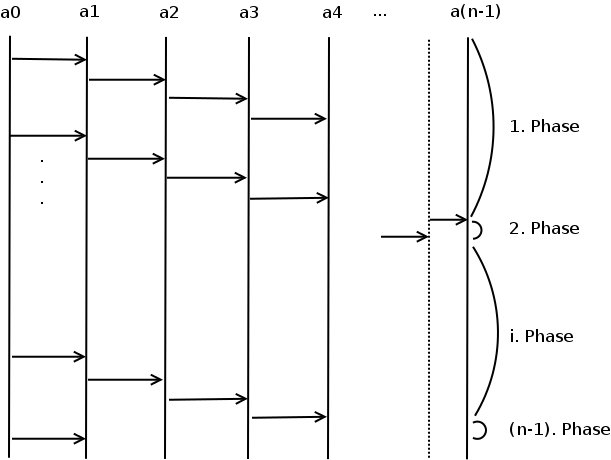
\includegraphics[width=0.8\linewidth]{1/Grafik/Bubblesort.png}
\caption{Bubblesort}
\end{center}
\end{figure}


\subsection{Pseudocode}
\begin{lstlisting}
void bubblesort (int[] a) {
  int n = a.length;
  for (int i = 1; i < n; i++) {
    for (int j = 0; j < n-i; j++) {
      if ( a[j] < a[j+1])
        swap (a, j, j+1);
    }
  }
}
\end{lstlisting}
\paragraph{Schleifen-Invariante:} Nach dem Ablauf der i-ten Phase gilt:
\begin{center}
	Die Feldpositionen n-i,\ldots,n-i enthalten die korrekt sortierten Feldelemente
\end{center}
\paragraph{Beweis} durch Induktion nach i $\overset{i=n-1}{\Longrightarrow}$ Sortierung am Ende korrekt.


\pagebreak

\subsection{Laufzeitanalyse}

$T(n) =$ Zahl der durchgeführten Elementvergleiche für eine Eingabemenge von n Elementen\\

\begin{tabular}{rcc}
	1.&Phase & n-1 \\
	2.&Phase & n-1 \\
	3.&Phase & n-1 \\
	 & $\vdots$ &  \\
	i.& Phase & n-1 \\
	 & $\vdots$ &  \\
	(n-1).&Phase & n-1 \\ \hline
	\multicolumn{3}{c}{$1+2+3+\ldots+(n+1)$}
\end{tabular}
\[ T(n)=\sum_{i=1}^{n-1} i = \frac{n(n-1)}{2}\in O(n^2) \]
\begin{tabular}{c|c}
	$n$ & $T_{real}$ \\ \hline
	$2^{10}$ & 8ms \\
	$2^{11}$ & 11ms \\
	$2^{12}$ & 26ms \\
	$\vdots$ &  \\
	$2^{16}$ & 5,819s \\
	$2^{17}$ & 23,381s \\
	$\vdots$ &  \\
	$2^{20}$ & 16min \\
	$\vdots$ &  \\
	$2^{26}$ & 52d 
\end{tabular}
\[ T_{real}(n)\approx cn^2~~ c\approx10^{-6}\]
\[T_{real} (2n) \approx c \cdot (2n)^2 = 4 cn^2 = 4T_{real}(n) \]
\[\frac{T_{real}(2n)}{T_{real}(n)} = 4 \]



\section{Heapsort}
\paragraph{z.B.} \begin{tabular}{ccccccccccccccc}
	21&6&4&7&12&5&3&11&14&17&19&8&9&10&42
\end{tabular}

%hier dürfen gerne noch die einzelnen Schritte als Grafik eingefügt werden

\subsection*{Skizze}
\begin{figure}[h]
%\begin{center}
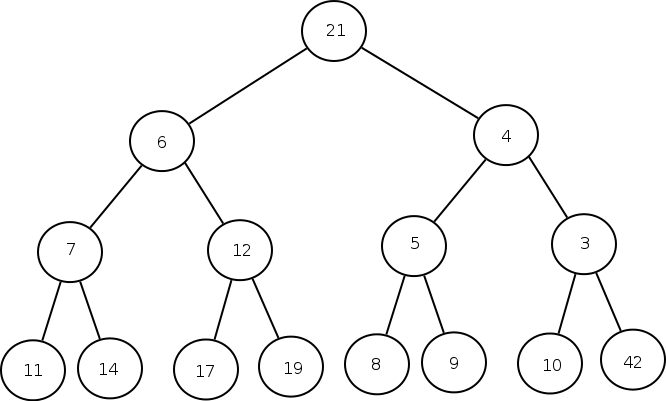
\includegraphics[width=0.3\linewidth]{1/Grafik/heap1.png}
\captionsetup{labelsep=space,justification=justified,singlelinecheck=off}
\caption{Heapsort (Ausgangssituation)}
%\end{center}
\end{figure}

\newpage

\subsection*{Indices innerhalb der Baumstruktur}
\begin{flalign*}
&\lfloor \frac{i-1}{2} \rfloor&
\end{flalign*}

\begin{figure}[h]
\vspace{-45pt}
\hspace{35pt}
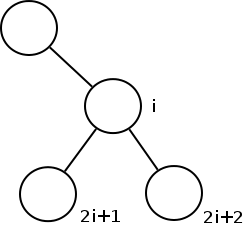
\includegraphics[width=0.2\linewidth]{1/Grafik/HeapAufbau.png}
\caption{Indices}
\end{figure}


\subsection*{Heap-Eigenschaft}

\begin{figure}[h]
\begin{center}
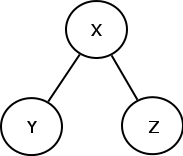
\includegraphics[width=0.2\linewidth]{1/Grafik/HeapEigenschaft.png}\\
$x \geq y$\\
$x \geq z$
\caption{Heap-Eigenschaft}
\end{center}
\end{figure}


\subsection{Idee}
\paragraph{Phase 1} Stelle die Heap-Eigenschaft überall her\\
$\Rightarrow$ größtes Element steht in der Wurzel
\paragraph{Phase 2} Tausche Wurzel mit letztem Feldelement\\
(z.B. 42 mit 3)\\
- Entferne letztes Feldelement aus dem Baum\\
- Gehe erneut zu Phase 1

\chapter{Vorlesung 2}
\section*{Heapsort (Fortsezung)}
%Grafik
\begin{lstlisting}
heapify ( int[] a, int i, int n) {
  while (2i + 1 < n) {		//linkes Kind von i existiert
    int j = 2i + 1;
    if ( 2i +2 < n)  		//rechtes Kind von i existiert
      if ( a[j] < a[j+1])
        j = j + 1;  		//j steht für Indes des größten Kindes
    if ( a[i] > a[j])  		//Vater größer als Kind
      break;  			//Abbruch, weil heap bereits erfüllt
    swap(a,i,j); 		//Tausch zwischen Vater und Kind
    i = j;
  }
}
\end{lstlisting}
%Geht weiter
\chapter{Vorlesung 11}
\section{AVL-Bäume von Adelson-Velskii and Landis}
\begin{wrapfigure}[2]{l}{0.3\linewidth}
	\vspace{-50pt}
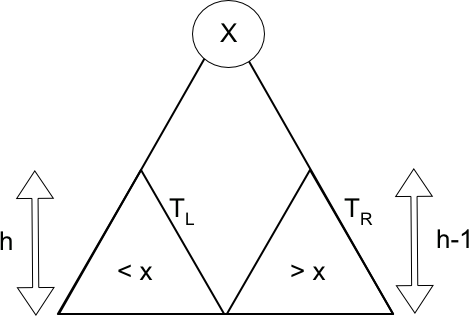
\includegraphics[width=\linewidth]{11/Grafik/img1.png}
\caption{}
\end{wrapfigure}

\vspace{30pt}
\paragraph{Ziel:}%
Zeige, dass die maximale Tiefe eines AVL-Baums mit n Knoten ($\hat{=}~ n$ gespeicherten Schlüsseln) $O(\log(n))$ beträgt.
\vspace{50pt}
\subsection{AVL-Eigenschaft:} 
$|h(T_L)-h(T_R)| \leq 1$ muss für jeden Knoten des Baums gelten. $~~~\Rightarrow$ Suchzeit $O(\log(n))$ im worst case.\\
\begin{wrapfigure}{l}{0.3\linewidth}
	\vspace{40pt}
	
\includegraphics[width=\linewidth]{11/Grafik/img2.png}
	\caption{}
	\vspace{500pt}
\end{wrapfigure}

$n(h) =$ minimale Anzahl von Knoten in AVL-Baum der Tiefe h
\[n(h) \geq 1+n(h-2) + n(h-1)\text{ mit  }n(0)=0\text{ und }n(1)=1\]
\[n \geq f(h)\footnote{$f(h)$ meint hierbei die h-te Fibonacci-Zahl} = \frac{1}{\sqrt{5}} \cdot (\phi^h-\phi^{-h})\text{ mit}\] 
\[\phi = \frac{1+\sqrt{5}}{2} \approx 1,61\ldots\]
\[\Rightarrow n \geq c \cdot \phi^h\]
\[\Leftrightarrow h \leq \log{(\frac{n}{c})}\]
\[\Rightarrow h \in O(\log{n})\]
\begin{flushright}
	q.e.d.
\end{flushright}
\clearpage

\section{Rotationen}

\begin{figure}[H]
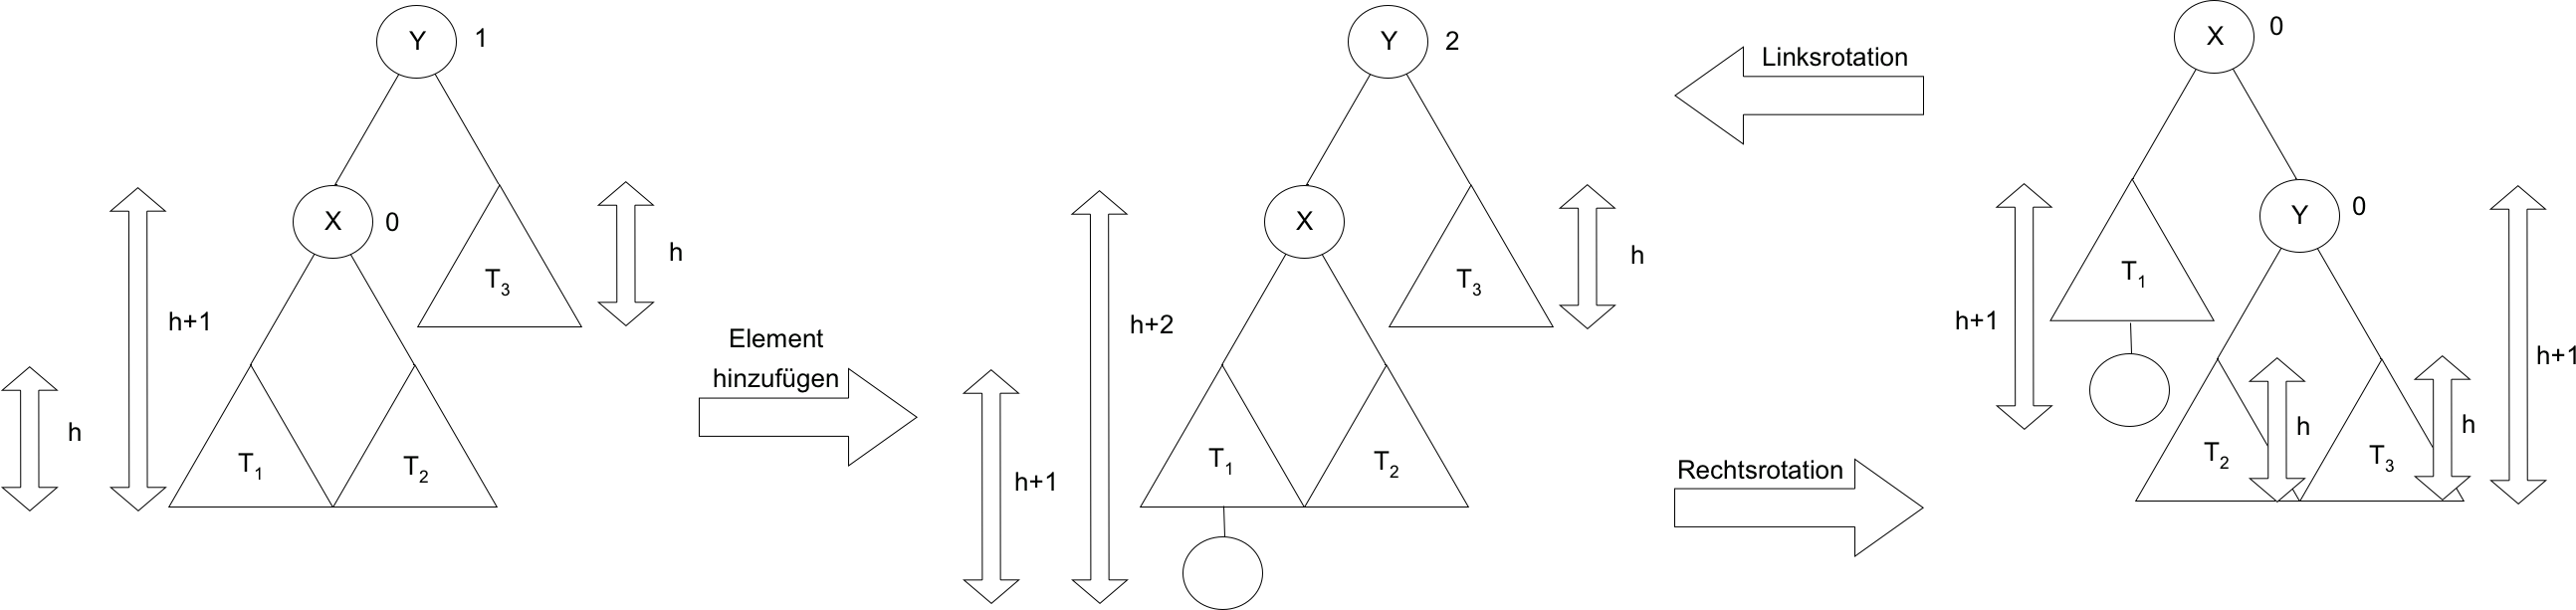
\includegraphics[width=\textwidth,left]{11/Grafik/img3_Rotation.png}
$Keys(T_1) < Key(X) < Keys(T_2) < Key(Y) < Keys(T_3)$ \\
\lstinline[language=Java]{balance(Y) = height(Y.left)-height(Y.right)}
\end{figure}

\begin{wrapfigure}{l}[-18pt]{0.24\textwidth}
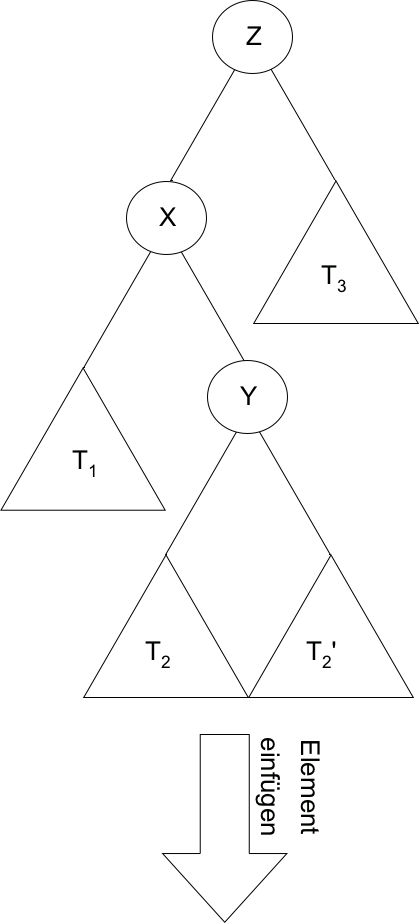
\includegraphics[width=\linewidth]{11/Grafik/img4_doppelRotation_1.png}
\end{wrapfigure}

$Keys(T_1) < Key(X) < Keys(T_2) < Key(Y) < Keys(T_2^{'}) < Key(Z) < Keys(T_3)$

\begin{figure}
	\begin{subfigure}[H]{0.3\textwidth}
		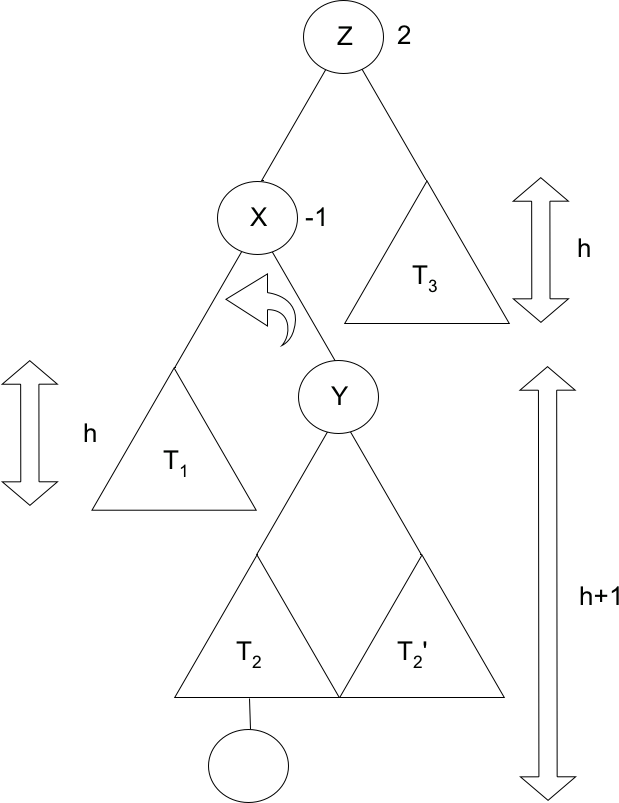
\includegraphics[width=\linewidth]{11/Grafik/img5_doppelRotation_2.png}
	\end{subfigure}
	\begin{subfigure}[H]{0.3\textwidth}
			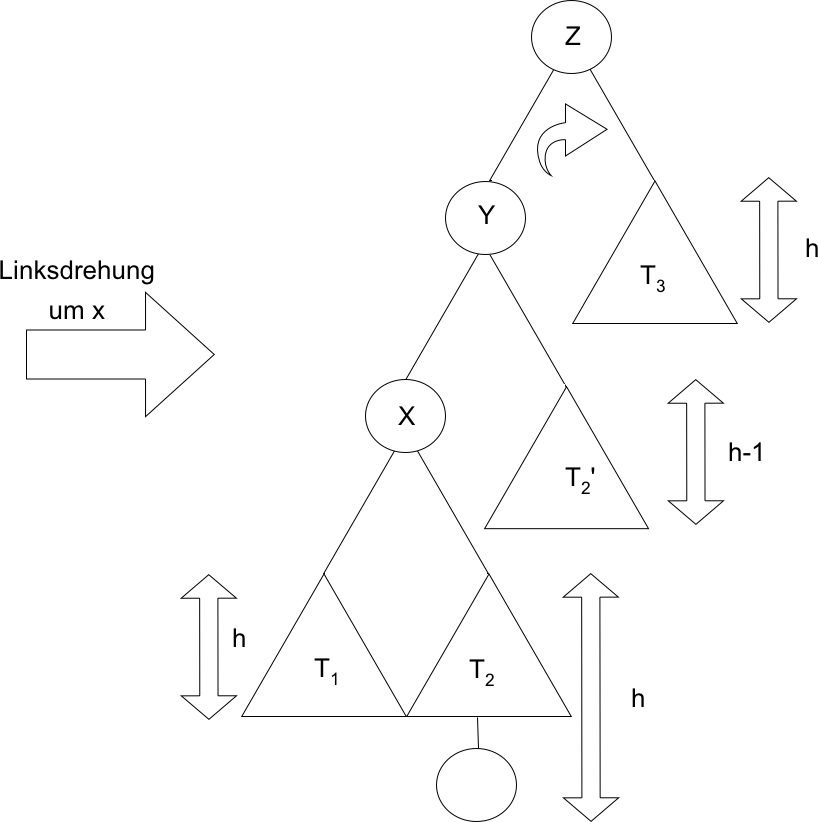
\includegraphics[width=\linewidth]{11/Grafik/img6_doppelRotation_3.png}
	\end{subfigure}
	\begin{subfigure}[H]{0.4\textwidth}
				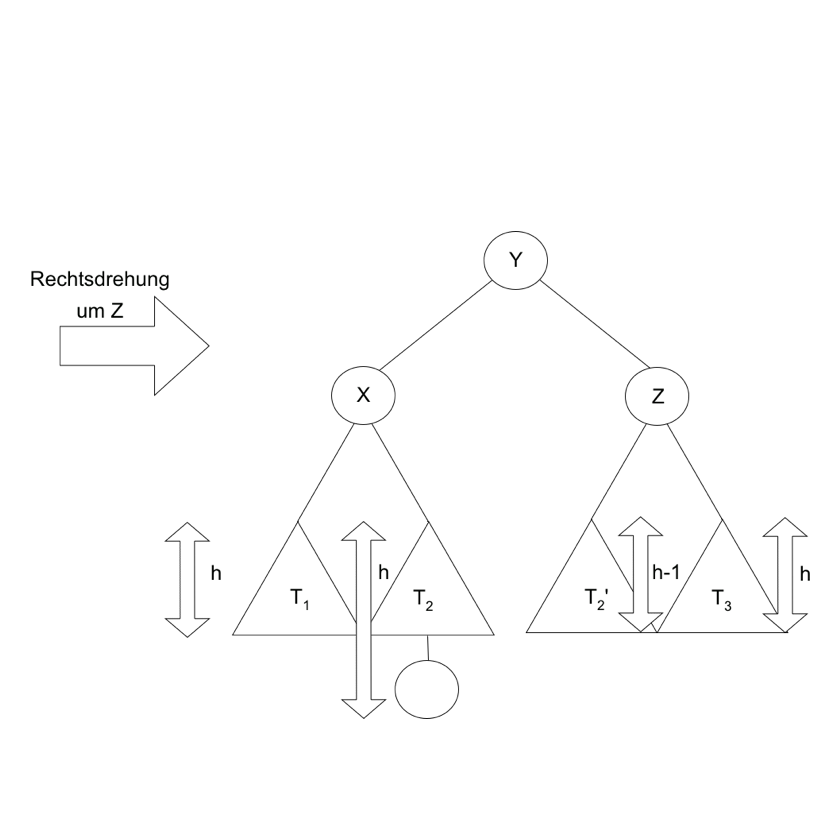
\includegraphics[width=\linewidth]{11/Grafik/img7_doppelRotation_4.png}
	\end{subfigure}
\end{figure}

\clearpage


\section{Pseudo-Code}
\lstinputlisting[language=Java]{11/Code/Node.java}

\paragraph{Anmerkung:} Die Laufzeit des Einfügens bleibt in $O($Baumtiefe$)$ = $O(\log{n})$. Nur einer der vier Fälle ist notwendig, um die Balance herzustellen. 
\pagebreak
\part{Vorlesung 12}
\section{(a,b)-Suchbäume}
Blattorientierte Speicherung der Elemente\\
Innere Knoten haben mindestens a und höchstens b Kinder und tragen entsprechende Schlüsselwerte, um die Suche zu leiten.
\paragraph{Beispiel:}%%2 Bilder einfügen
\[h\hat{=}\text{Tiefe}\Rightarrow ~~ a^h\leq n \leq b^h ~\Rightarrow ~ \log_b n \leq h \leq \log_a n\]
%Bilder
\subsection{Aufspaltung bei Einfügen}
%Bilder
\subsection{Verschmelzen von Knoten beim Löschen}
%Bilder
Aufspalte- und Verschmelze-Operationen können sich von der Blattebene bis zur Wurzel kaskadenartig fortpflanzen. Sie bleiben aber auf den Suchpfad begrenzt.\\
$\Rightarrow$ Umbaukosten sind beschränkt durch die Baumtiefe $=O(\log n)$
\section{Amortisierte Analyse}
\paragraph{Beispiel: Binärzähler}
	\begin{tabular}{lr}
		$000$& \\
		$001$&$\text{Kosten}(1)=1$\\
		$010$&$=2$\\
		$011$&$=1$\\
		$100$&$=3$\\
		$101$&$=1$\\
		$110$&$=2$\\
		$111$&$=1$\\
		 &$\overline{11}$
	\end{tabular}
	Kosten der Inkrement-Operation $\hat{=}$ Zahl der Bit-Flips\\
	Naive Analyse $2^k=n$
	\[1\cdot\frac{n}{2}+2\cdot\frac{n}{4}+3\cdot\frac{n}{8}+\ldots+k\cdot\frac{n}{2^k}=\frac{n}{2}\sum_{i=1}^{k}i(\frac{1}{2})^{i-1}=2^{k+1}-k-2=2n-k-2 \]
Von $0$ bis $n$ im Binärsystem zu zählen kostet  $\leq 2n$ Bit-Flips
\paragraph{Sprechweise:} amortisierte Kosten einer Inkrement-Operation sind $2$\\
Folge von n-Ops kostet $2n$
\subsection{Bankkonto-Methode}
\[\text{Konto}(i+1)=\text{Konto}(i)-\text{Kosten}(i)+\text{Einzahlung}(i) \]
\[\sum_{i=1}^{n}\text{Kosten}(i)=\text{tatsächliche Gesamtkosten} = \sum_{i=1}^{n}(\text{Einzahlung}(i)+\text{Konto}(i-\text{Konto}(i+1))\]
\[=\sum_{i=1}^{n}\text{Einzahlung}(i)+\text{Konto}(1)-\text{Konto}(n+1) \]
	\begin{tabular}{lr}
		$000$& \\
		$001_\text{\euro}$&$\text{Kosten}(1)=1$\\
		$01_\text{€}0$&$=2$\\
		$01_\text{€}1_\text{€}$&$=1$\\
		$1_\text{€}00$&$=3$\\
		$1_\text{€}01_\text{€}$&$=1$\\
		$1_\text{€}1_\text{€}0$&$=2$\\
		$1_\text{€}1_\text{€}1_\text{€}$&$=1$\\
		&$\overline{11}$
	\end{tabular}
	\subsubsection{Kontoführungsschema: für Binärzähler}
	1€ pro 1 in der Binärdarstellung\\
	Jeder Übergang $1_\text{€}\rightarrow0$ kann dann mit dem entsprechenden Euro Betrag auf dieser 1 bezahlt werden.\\
	Es gibt pro Inkrement Operation nur einen $0\rightarrow1$ Übergang\\
	2€ Einzahlung für jede Inc-Operation reichen aus um:
	\begin{enumerate}
		\item diesen $0\rightarrow1$ Übergang zu bezahlen
		\item die neu entstandene $1_\text{€}$ mit einem Euro zu besparen.
	\end{enumerate}
	\[\text{GK} = 2(2^k-1)+0\footnote{Zählerstand(000)}-k\footnote{Zählerstand($\overbrace{111\ldots1}^k$)}=2n-k-2\]


\chapter{Vorlesung 13}
\satz Ausgehend von einem \underline{leeren} 2-5-Baum betrachten wir die Rebalancierungskosten $C$ (Split- und Fusionsoperationen) für eine Folge von $m$ Einfüge- oder Löschoperationen. Dann gilt: $C\in O(m)$\\
d.h. Amortisierte Kosten der Split- und Fusionsopeartionen sind konstant.\\
! Dies bezieht sich nicht auf die Suchkosten, die in $O(\log n)$ liegen.
\paragraph*{Beweisidee:}
\subparagraph*{Kontoführung:}
\begin{tabular}{|c|c|c|c|c|c|}
	\hline \rule[-2ex]{0pt}{5.5ex} 1 & 2 & 3 & 4 & 5 & 6 \\ 
	\hline \rule[-2ex]{0pt}{5.5ex} 2€ & 1€ & 0€ & 0€ & 1€ & 2€ \\ 
	\hline 
\end{tabular} \\
regelmäßige Einzahlung: 1€\\
Durch eine Einfüge- oder Löschoperation steigt oder fällt der Knotengrad des direkt betroffenen Knotens um höchstens 1. $\Rightarrow$ 1€ Einzahlung reicht zur Aufrechterhaltung dieses Sparplanes.\\
Jetzt Beseitigung der temporären 1- und 6-Knoten:\\
Ein 6-Knoten nutzt 1€ um seinen Split zu bezahlen. Die beiden neu entstehenden 3-Knoten benötigen kein Kapital. Der Vaterknoten des gesplitteten 6-Knotens benötigt ggf. den zweiten verfügbaren €.\\
Analoge Betrachtung für Fusion eines temp. 1-Knotens.
\section{Hashing}
\begin{figure}[h]
\centering
\caption[Universum und Hashtabelle der Größe m]{Universum und Hashtabelle der Größe m}
\label{fig:hashing}
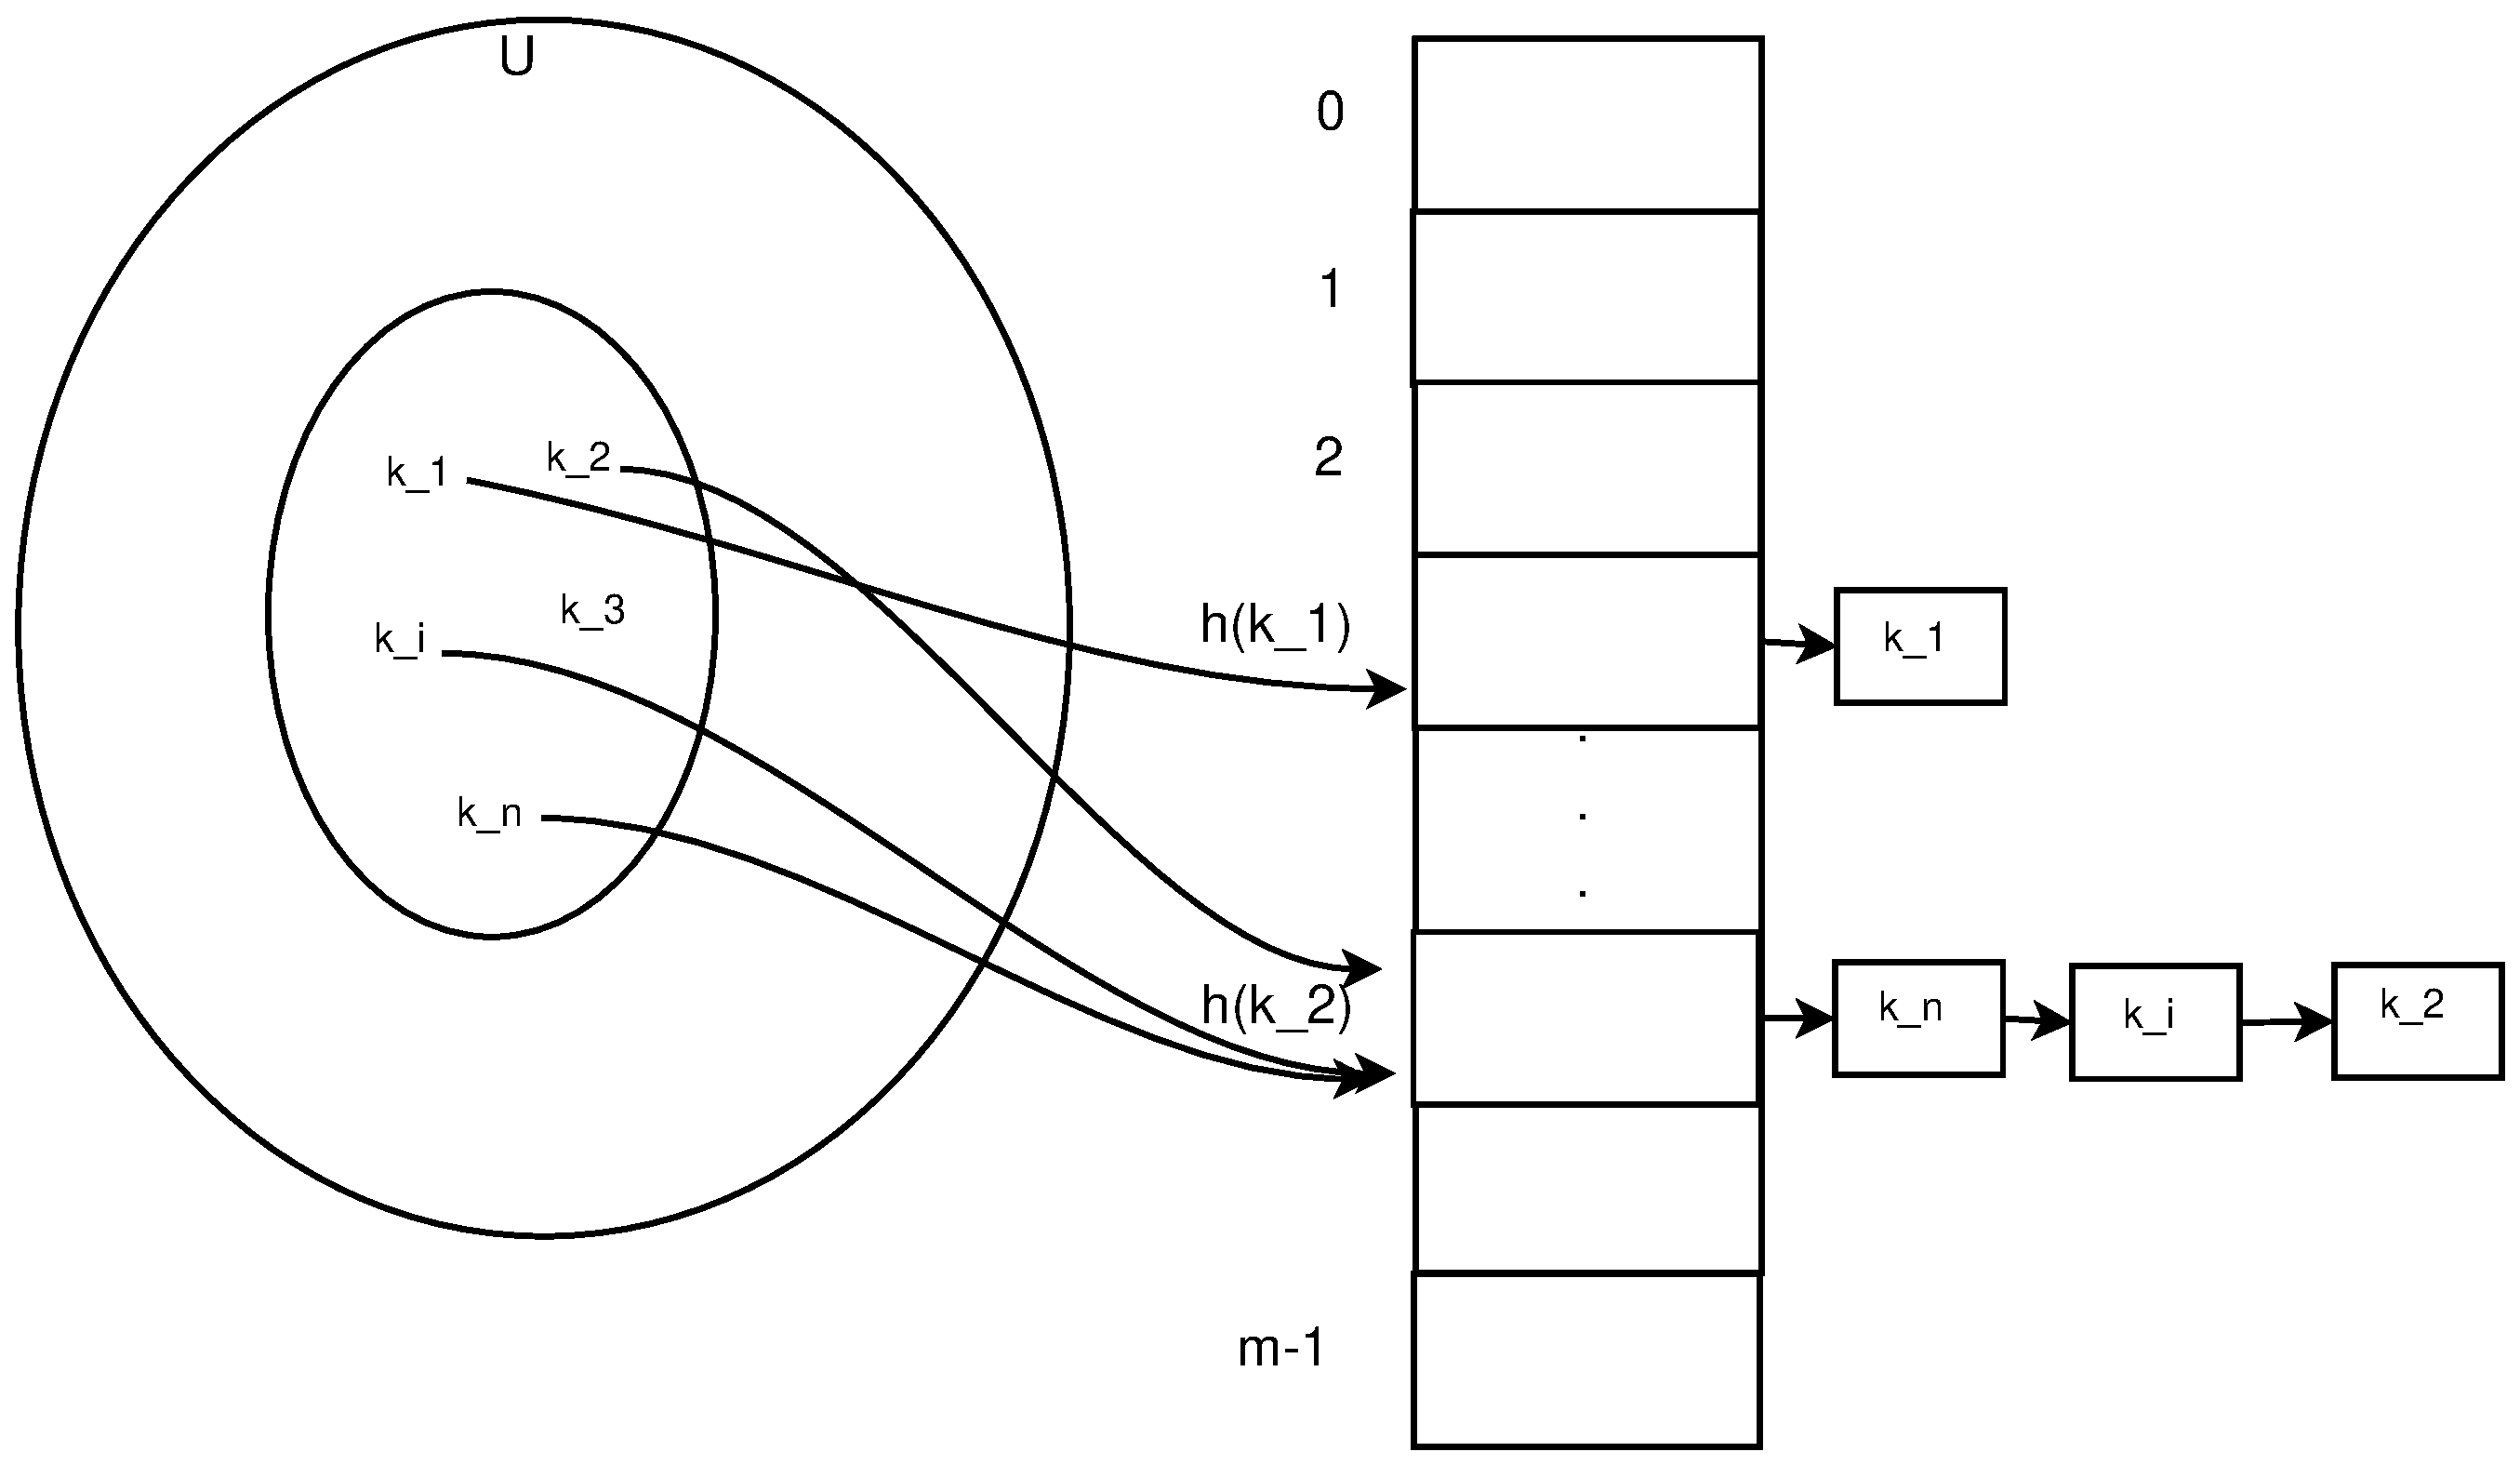
\includegraphics[width=0.8\linewidth]{13/Grafik/hashing}
\end{figure}
$U \subseteq \mathbb{N}$ z.B. 64-Bit-Integer\\
$n=$ Zahl dr zu verwaltenden Schlüssel\\
\[|U| >> n\]
Hashfunktion h:
\[h: U\rightarrow[0,\ldots,m-1]\]
\[\text{z.B. }k\mapsto k \mod m \]
Einfache Annahme: (einfaches uniformes Hashing)
\[\forall~k_i,k_j \in U : Pr(h(k_i)=h(k_j))=\frac{1}{m}   \]
\subsubsection{Analyse der Laufzeit zum Einfügen eines neuen Elementes k}
\begin{itemize}
	\item $h(k)$ berechnen $\longrightarrow O(1)$
	\item Einfügen am Listenanfang in Fach $h(k)$. $\longrightarrow O(1)$
\end{itemize}
\subsubsection{Analyse der Suchzeit für einen Schlüssel $k$}
\begin{itemize}
	\item $h(k)$ $\longrightarrow O(1)$
	\item Listenlänge zum Fach $h(k)$ sei $n_{h(k)}$ also beim Durchlauf der kompletten Liste $\longrightarrow O(n_{h(k)})$
\end{itemize}
\[ E(n_{h(k)})=\frac{n}{m}=\alpha\footnote{Belegungsfaktor} \]
\[ \text{Suchzeit}(\text{Einfügen})\in O(1+\alpha) \]
\subsubsection{Laufzeit beim Löschen von Schlüssel $k$}
\begin{itemize}
	\item $h(k) \longrightarrow O(1)$
	\item Durchlaufen der Liste $\longrightarrow 0(n_{h(k)})$
	\item Löschen durch "`Pointer-Umbiegen"' $\longrightarrow O(1)$
\end{itemize}
\subsection{Universelles Hashing}
\paragraph*{Idee} Arbeite nicht mit einer festen Hashfunktionm sondern wähle am Anfang eine zufällige Hashfunktion aus einer Klasse von Hashfunktionen aus.
\paragraph*{z.B.} \[ h_{a,b}(k)=((a\cdot k +b) mod p) mod m \]
p sei eine hinreichend große Primzahl$~~~~0<a<p, 0\leq b < p$
\[ \mathcal{H}_{p,m}=\{ h_{a,b}(k) | 0 < a < p, ~ 0 \leq b < p \} \]
\[ |\mathcal{H}_{p,m}| = p(p-1) \]
\paragraph*{Definition} $\mathcal{H}$ heißt universell $\Leftrightarrow~~\forall~k,l\in U:~ Pr(h(k)=h(l))\leq \frac{1}{m}$
\paragraph*{Suchzeit}
\[ \mathcal{X}_{k,l}=\begin{cases}1&\text{für }h(k)=h(l)\\0&\text{sonst}\end{cases} \]
\[ E(n_{h(k)})=E\left( \sum_{l \in T, l \neq k} \right) =  \sum_{l \in T, l \neq k} E(X_{k,l}) =  \sum_{l \in T, l \neq k} Pr(h(k)=h(l)) = \sum_{l \in T, l \neq k} \frac{1}{m} = \frac{n-1}{m} = \alpha \] 
\chapter{Vorlesung}
\section*{Universelles Hashing (Fortsetzung)}
Könnte ein boshafter Mitspieler n Schlüssel bei gegebener fester Hashfunktion wählen, so würde er solche wählen, die auf den gleichen Slot unter gegebener Hashfunktion abgebildet werden. $\rightsquigarrow$ Durchschnittliche Ablaufzeit von $O(n)$
\paragraph{Idee} zufällige Wahl der Hashfunktion aus einer Familie von Funktionen derart, dass die Wahl unabhängig von den zu speichernden Schlüssel ist (universelles Hashing).
\subsection{Definition}
Sei $\mathcal{H}$ eine endliche Menge von Hashfunktionen, welche ein gegebenes Universum $U$ von Schlüsseln auf $\{ 0,\ldots,m-1 \}$ abbildet. Sie heißt universell, wenn für jedes Paar von Schlüsseln $k,l\in U~~l\neq k$ die Anzahl der Hashfunktionen $h\in \mathcal{H}$ mit $h(l)=h(k)$ höchstens $\frac{|\mathcal{H}|}{m}$. Anders: Für ein zufälliges $h\in\mathcal{H}$ beträgt die Wahrscheinlichkeit, dass zwei unterschiedliche Schlüssel $k,l$ kollidieren nicht mehr als $\frac{1}{m}$ ist.
\subsection{Beispiel}
$p$ Primzahl, so groß, dass alle möglichen Schlüssel $k\in U$ im $0,\ldots,p-1$ liegen. $\mathbb{Z}/p\mathbb{Z}$ bezeichnet den Restklassenring $\mod{p}$ (weil $p$ prim, ist $\mathbb{Z}/p\mathbb{Z}$ ein Körper).
$\mathbb{Z}/p\mathbb{Z}^*$ ist die Einheitengruppe.
\paragraph{Annahme:} Die Menge der Schlüssel im Universum $U$ ist größer als die Anzahl der Slots in der Hashtabelle. Für $a\in \mathbb{Z}/p\mathbb{Z}^*$ und $b\in \mathbb{Z}/p\mathbb{Z}$ betrachte:
\[ h_{a,b}(k) := (a\cdot k + b \mod{p})\mod{m} ~~~(*)\]
Damit ergibt sich die Familie
\[ \mathbb{Z}/p\mathbb{Z}^*=\{ 1,\ldots,p-1 \}~~\mathbb{Z}/p\mathbb{Z}=\{ 0,\ldots,p-1 \}~~ \mathcal{H}_{p,m}=\{h_{a,b}|a\in \mathbb{Z}/p\mathbb{Z}^*, b \in\mathbb{Z}/p\mathbb{Z}^{(*)}~~|\mathcal{H}|=p(p-1)  \} \]
\paragraph{Satz}
Die in $(*)$ eingeführte Klasse von Hashfunktionen ist universell.
\paragraph{Beweis}
Seien $k,l$ Schlüssel auf $\mathbb{Z}/p\mathbb{Z}$ mit $k\neq l$\\
Für $h_{a,b}\in \mathcal{H}_{p,m}$ betrachten wir
\[ r=(a\cdot k+b)\mod{p} \]
\[ s=(a\cdot l+b)\mod{p} \]
Es ist $r \neq s$\\
Dazu:
\[ r-s = a\cdot(k-l) \mod{p} ~~~(*2)\]
\paragraph{Angenommen $r-s=0$}
\[ 0=a\cdot(k-l)\mod{p}\text{, aber }a\in\mathbb{Z}/p\mathbb{Z}^* \Rightarrow a\neq 0\text{ und } k\neq l \Rightarrow k-l\neq 0 \]
Da $p$ prim ist $\mathbb{Z}/p\mathbb{Z}$ ein Körper $\Rightarrow$ kein Nullteiler $\Rightarrow a\cdot (k-l)\neq 0\Rightarrow r\neq s$\\
Daher bilden $h_{a,b}\in \mathcal{H}_{p,m}$ unterschiedliche Schlüssel $k,l$ auf unterschiedliche Elemente ab. ("`Auf dem level $\mod{p}$"' gibt es keine Kollisionen).\\
Aus $(*2)$ folgt:
\[ (r-s)(k-l)^{-1} = a\mod{p} \]
\[ r-a\cdot k = b\mod{p} ~~\text{Bijektion zwischen (k,l) und (a,b)}\]
Daher ist die Wahrscheinlichkeit, dass zwei Schlüssel $h\neq l$ kollidieren, gerade die Wahrscheinlichkeit, dass $r\equiv s \mod{m}$, falls $r\neq S$ zufällig gewählt (aus $\mathbb{Z}/p\mathbb{Z}$).\\
Für gegebenes $r$ gibt es unter den übrigen $p-1$ Werten für $s$ höchstens $\lceil \frac{p-1}{m} \rceil \leq \lceil \frac{p}{m} \rceil -1$ Möglichkeiten, sodass $s\neq r\mod{p}$ aber $r=s\mod{m}$
\subsection{Abschätzung nach oben}
\[\lceil \frac{p}{m} \rceil -1  \leq \frac{(p+m-1)}{m}-1 = \frac{p-1}{m} \text{ Kollisionsmöglichkeiten} \]
Die Wahrscheinlichkeit, dass $r$ und $s$ kollidieren $\mod{m}$ Kollisionsmöglichkeiten / Gesamtzahl der Werte
\[ =\frac{p-1}{m}\cdot\frac{1}{p-1}=\frac{1}{m} \]
$\Rightarrow$ Für ein Paar von Schlüsseln $k,l\in \mathbb{Z}/p\mathbb{Z}$ mit $k\neq l$
\[ P[h_{a,b}(k)=h_{a,b}(l)] \leq \frac{1}{m} \Rightarrow \mathcal{H}_{p,m} \text{ universell!} \]
\section{Perfektes Hashing}
\paragraph{Wichtig}
Menge der Schlüssel ist im Vorhinein bekannt und ändert sich nicht mehr.
\paragraph{Beispiele}
reserved words bei Programmiersprachen, Dateinamen auf einer CD
\subsection{Definition}
Eine Hashmethode heißt perfektes Hashing, falls $O(1)$ Speicherzugriffe benötigt werden, um die Suche nach einem Element durchzuführen.
\paragraph{Idee}
Zweistufiges Hashing mit universellen Hashfunktionen.
\begin{enumerate}
	\item Schritt  $n$ Schlüssel, $m$ Slots durch Verwendung der Hashfunktion $h$, welche aus einer Familie universeller Hashfunktionen stammt.
	\item Schritt  Statt einer Linkedlist im Slot anzulegen, benutzen wir eine kleine zweite Hashtabelle $S_j$ mit Hashfunktion $h_j$
\end{enumerate}
\paragraph{Bild} Schlüssel $k=\{ 10, 22, 37, 49, 52, 60, 72, 75 \}$\\
Äußere Hashfunktion $h(k)=((a\cdot b) \mod{p})\mod{m}$
\[ a=3,~~b=42,~~p=101,~~m=9 \]
\[ h(10)= \underset{=72}{ \underbrace{ (3\cdot 10+42\mod101) } }\mod{9}=0 \]
\begin{figure}[h]
\centering
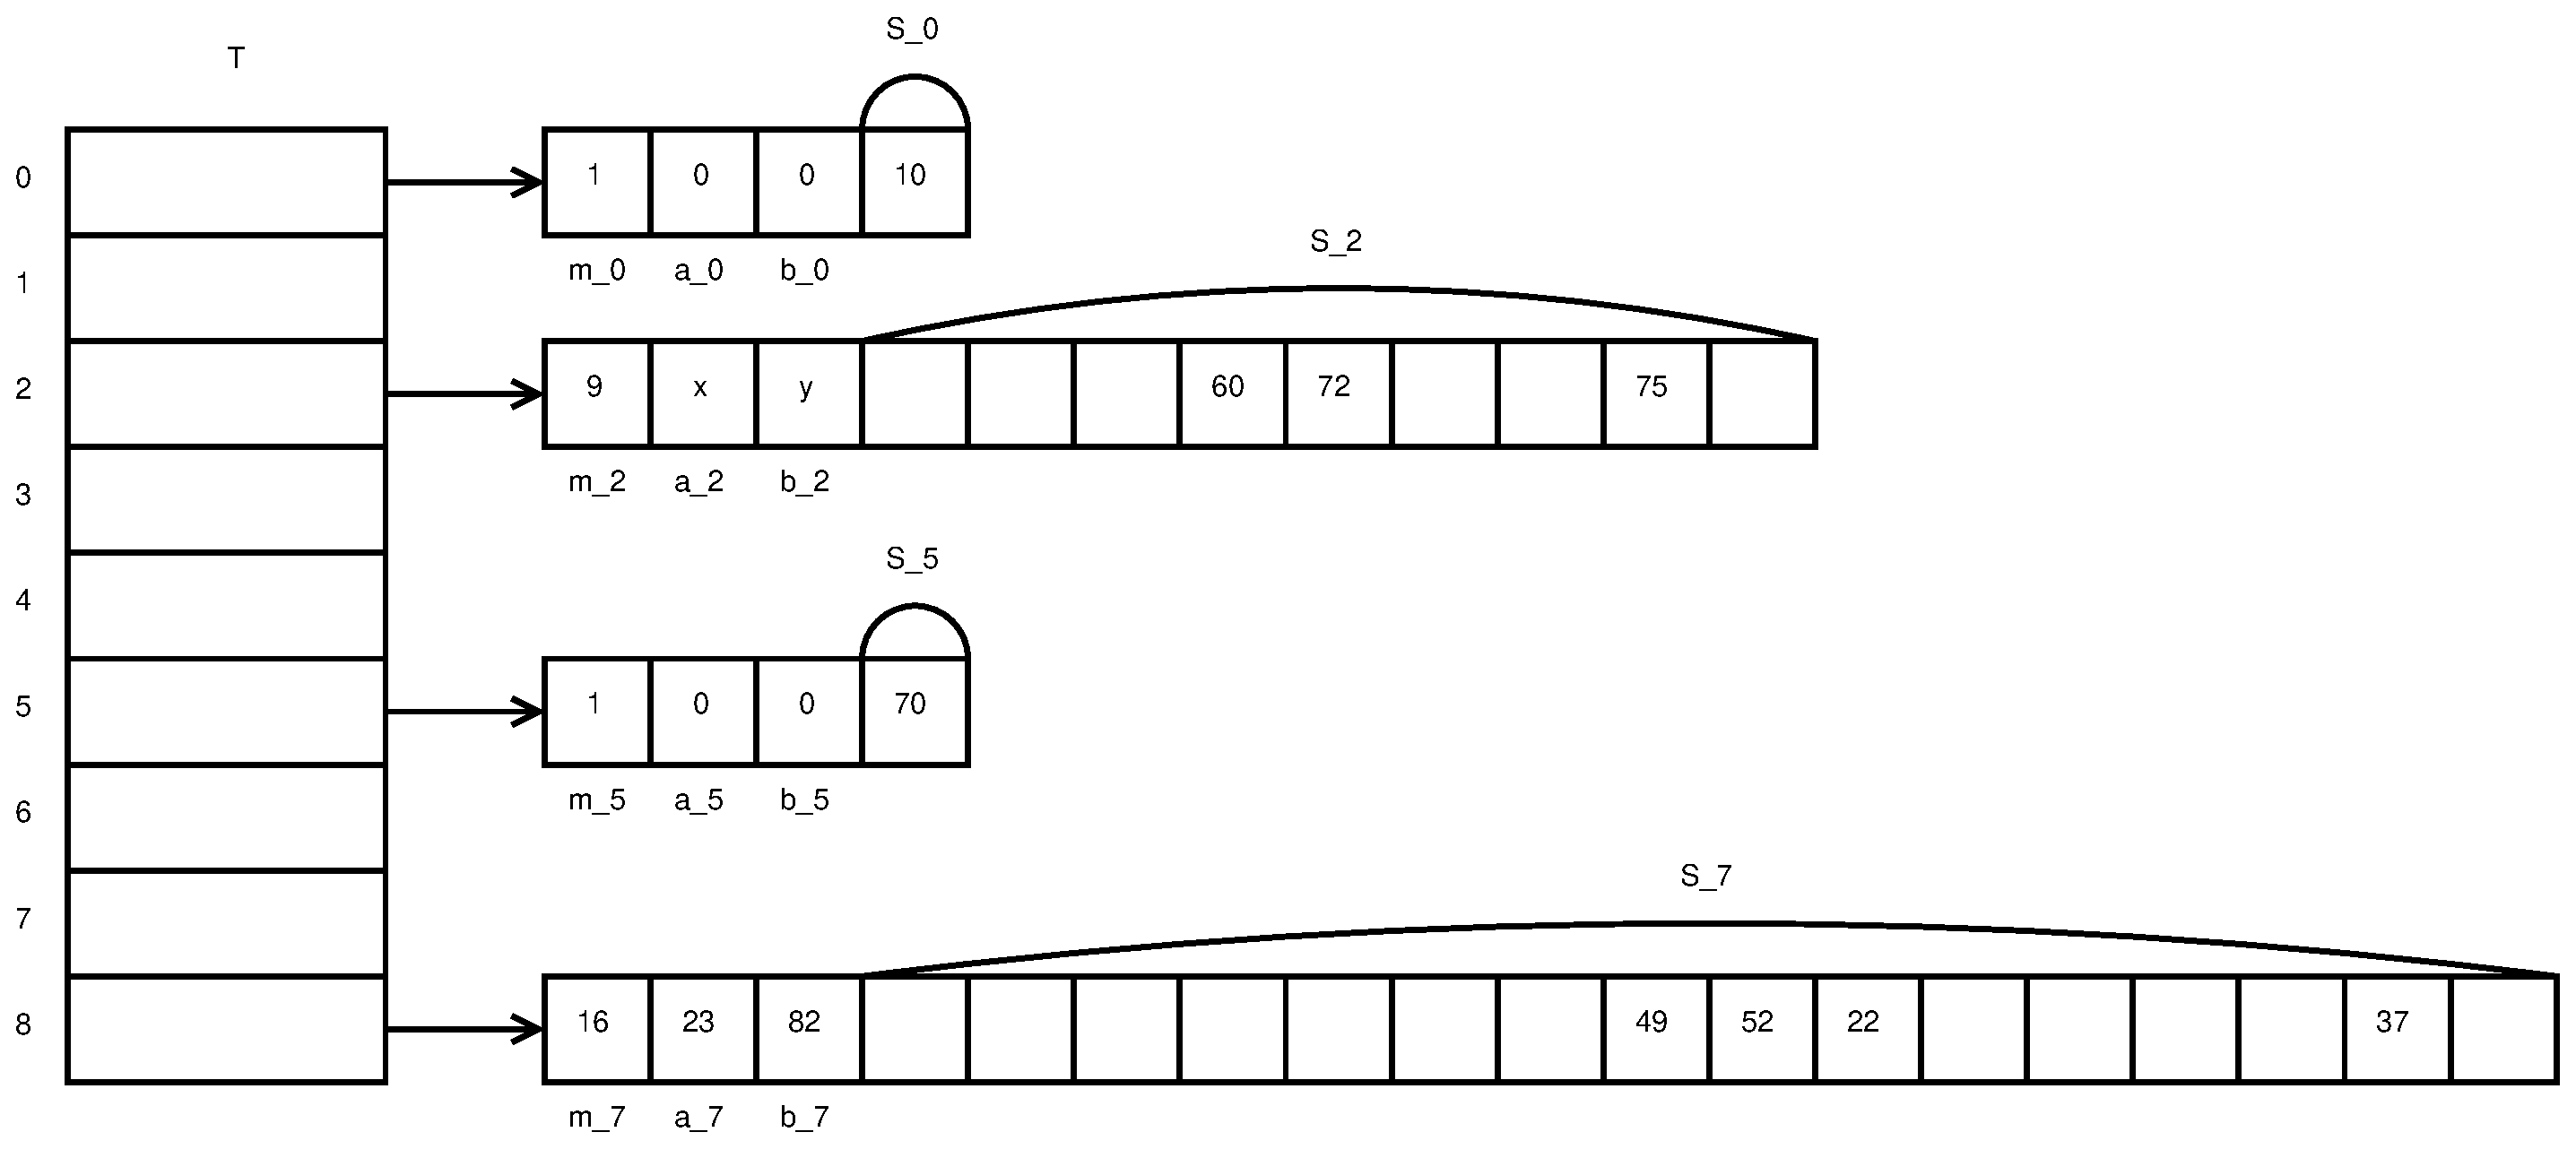
\includegraphics[width=0.7\linewidth]{14/Grafik/Hashing}
\caption{Perfekte Hashtabelle}
\label{fig:Hashing}
\end{figure}
Um zu garantieren, dass keine Kollision auf der zweiten Ebene auftreten, lassen wir die Größe von $S_j$ gerade $n_j^2$ sein ($n_j\neq \#$Schlüssel$\mapsto j$Slot).\\
Wir verwenden für die Hashfunktion der ersten Ebene eine Funktion aus $\mathcal{H}_{p,m}$. Schlüssel die im j-ten Slot werden in der sekundären Hashtabelle $S_j$ der Größe $m_j$ mittels $h_j$ gehasht.  $h_j\in\mathcal{H}_{p,m}$
\paragraph{Wir zeigen:} 2 Dinge:
\begin{enumerate}
	\item Wie versichern wir, dass die zweite Hashfunktion keine Kollision hat.
	\item Der erwartete Speicherbedarf ist $O(n)$
\end{enumerate}
\paragraph{zu 1.}
\subparagraph{Satz}
Beim Speichern von $n$ Schlüsseln in einer Hashtabelle der Größe $m=n^2$ ist die Wahrscheinlichkeit, dass eine Kollision auftritt $<\frac{1}{2}$
\subparagraph{Beweis:}
Es gibt $\binom{n}{2}$ mögliche Paare, die kollidieren können. Jedes kollidiert mit der Wahrscheinlichkeit $\leq \frac{1}{m}$, falls $h\in\mathcal{H}$ zufällig gewählt wurde.\\
Sei $X$ eine zufallsvariable(ZV), $X$ zählt Kollisionen:\\
Für $m=n^2$ ist die erwartete Zahl der Kollisionen:
\[ E[X]=\binom{n}{2}\cdot\frac{1}{m}=\binom{n}{2}\cdot\frac{1}{n^2}=\frac{n!}{2!(n-2)!n^2}=\frac{(n-1)}{2n}\leq\frac{1}{2} \]
Anwenden der Markow-Ungleichung (a=1):
\[ P[X\geq 1]\leq \frac{E[X]}{1}=\frac{1}{2} \Rightarrow \text{ Wahrscheinlichkeit für irgendeine Kollision ist } <\frac{1}{2} \]
\begin{flushright}
	q.e.d
	\end{flushright}
\subsection{Nachteil}
Für große $n$ ist $m=n^2$ nicht haltbar!
\paragraph{zu 2.}
Wenn die Größe der primären Hashtabelle $m=n$ ist, dann ist der Platzverbrauch in $O(n) \curvearrowright$ Betrachte Platzverbrauch der sekundären Hashtabellen.
\paragraph{Satz}
Angenommen wir wollen $n$ Schlüssel in einer Hashtabelle der Größe $m=n$ mit Hashfunktion $h\in \mathcal{H}$. Dann gilt:
\[ E\left[ \sum_{j=0}^{m-1} n_j^2 \right] <2n\]
\paragraph{Beweis}
\subparagraph{Betrachte}
\[ a^2= a+2\cdot\binom{a}{n}=a+2\cdot\frac{a^2-a}{2}~~~(*3) \]
\subparagraph{Betrachte}
\[ E\left[ \sum_{j=0}^{m-1} n_j^2\right] \overset{(*3)}{=} E \left[ \sum_{j=0}^{m-1} \left(n_j+2\binom{n_j}{2}\right) \right] \]
\[ \overset{lini. des EW}{=} E \left[ \underset{=n}{\underbrace{\sum_{j=0}^{m-1}n_j}} \right]+2E\left[ \sum_{j=0}^{m-1}\binom{n_j}{2} \right]=n+2E\left[ \sum_{j=0}^{m-1} \binom{n_j}{2}\right] \text{\# der Kollisionen}\]
Da unsere Hashfunktion universell ist, ist die erwartete Zahl dieser Paare:
\[ \binom{n}{2}\frac{1}{m}=\frac{n(n-1)}{2m}=\frac{n-1}{2}\text{, da }m=n \]
Somit
\[ E\left[ \sum_{j=0}^{m-1} n_j^2\right] \leq n+2\frac{n-1}{2}=2n-1<2n \]
\paragraph{Korollar}
Speichern wir $n$ Schlüssel in einer Hashtabelle der Größe $m=n$ mit einer zufälligen universellen Hashfunktion und setzen die Größe der Hashtabellen der zweiten Ebene auf $m_j=n_j^2$ für $j=0, m=1$, so ist der Platzverbrauch des perfekten Hashings weniger als $2n$. Die Wahrscheinlichkeit, dass der Platzverbrauch der zweiten Hashtabellen $\geq 4n$ ist, ist $\leq \frac{1}{2}$ ohne Beweis.
\chapter{Vorlesung 15}
Bei $n$ Elementen sollte die Hashtabelle $m=n^2$ groß sein.\\
Für die universellen Hashfunktionen \[\mathcal{H}_{p,m} = \{ h_{a,b}(k)=(a\cdot k + b) \mod{p} \mod{m}| 0<a<p,~0\leq b < p \}\]\\
$\binom{n}{1}$ Schlüsselpaare $(k,l)$ mit $k \neq l$
\[ E(\text{\#Kollisionen}) \leq \binom{n}{2}\cdot \frac{1}{m}\footnote{Universalität von $\mathcal{H}$}=\frac{n(n-1)}{2}\cdot\frac{1}{n^2}\leq\frac{1}{2} \]
\paragraph{Idee}
Zweistufiges Verfahren:
\begin{itemize}
	\item primäre Hashfunktion für Tabelle der Größe $m=n$
\end{itemize}
\begin{figure}[H]
\centering
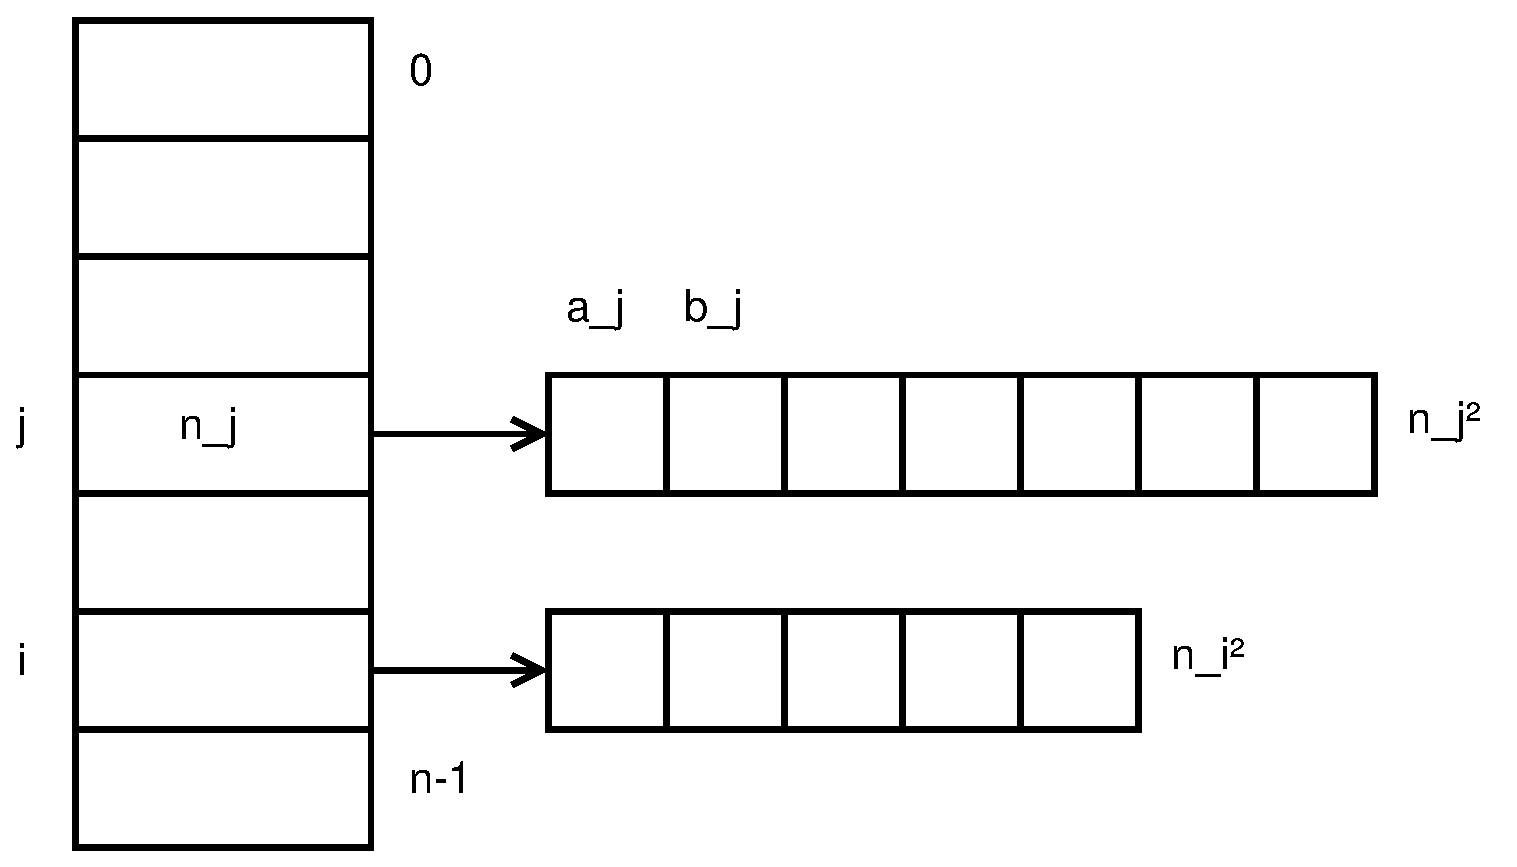
\includegraphics[width=0.5\linewidth]{15/Grafik/PHsching}
\caption[Perfektes Hashing]{Perfektes Hashing}
\label{fig:PHsching}
\end{figure}
\section{Graphen-Algorithmen}
\subsection{Einführung}
\[ G=(V,E)~~~V\text{ vertices, }E\text{ edges}~~~E\subseteq V \times V \]

\begin{figure}[H]
\centering
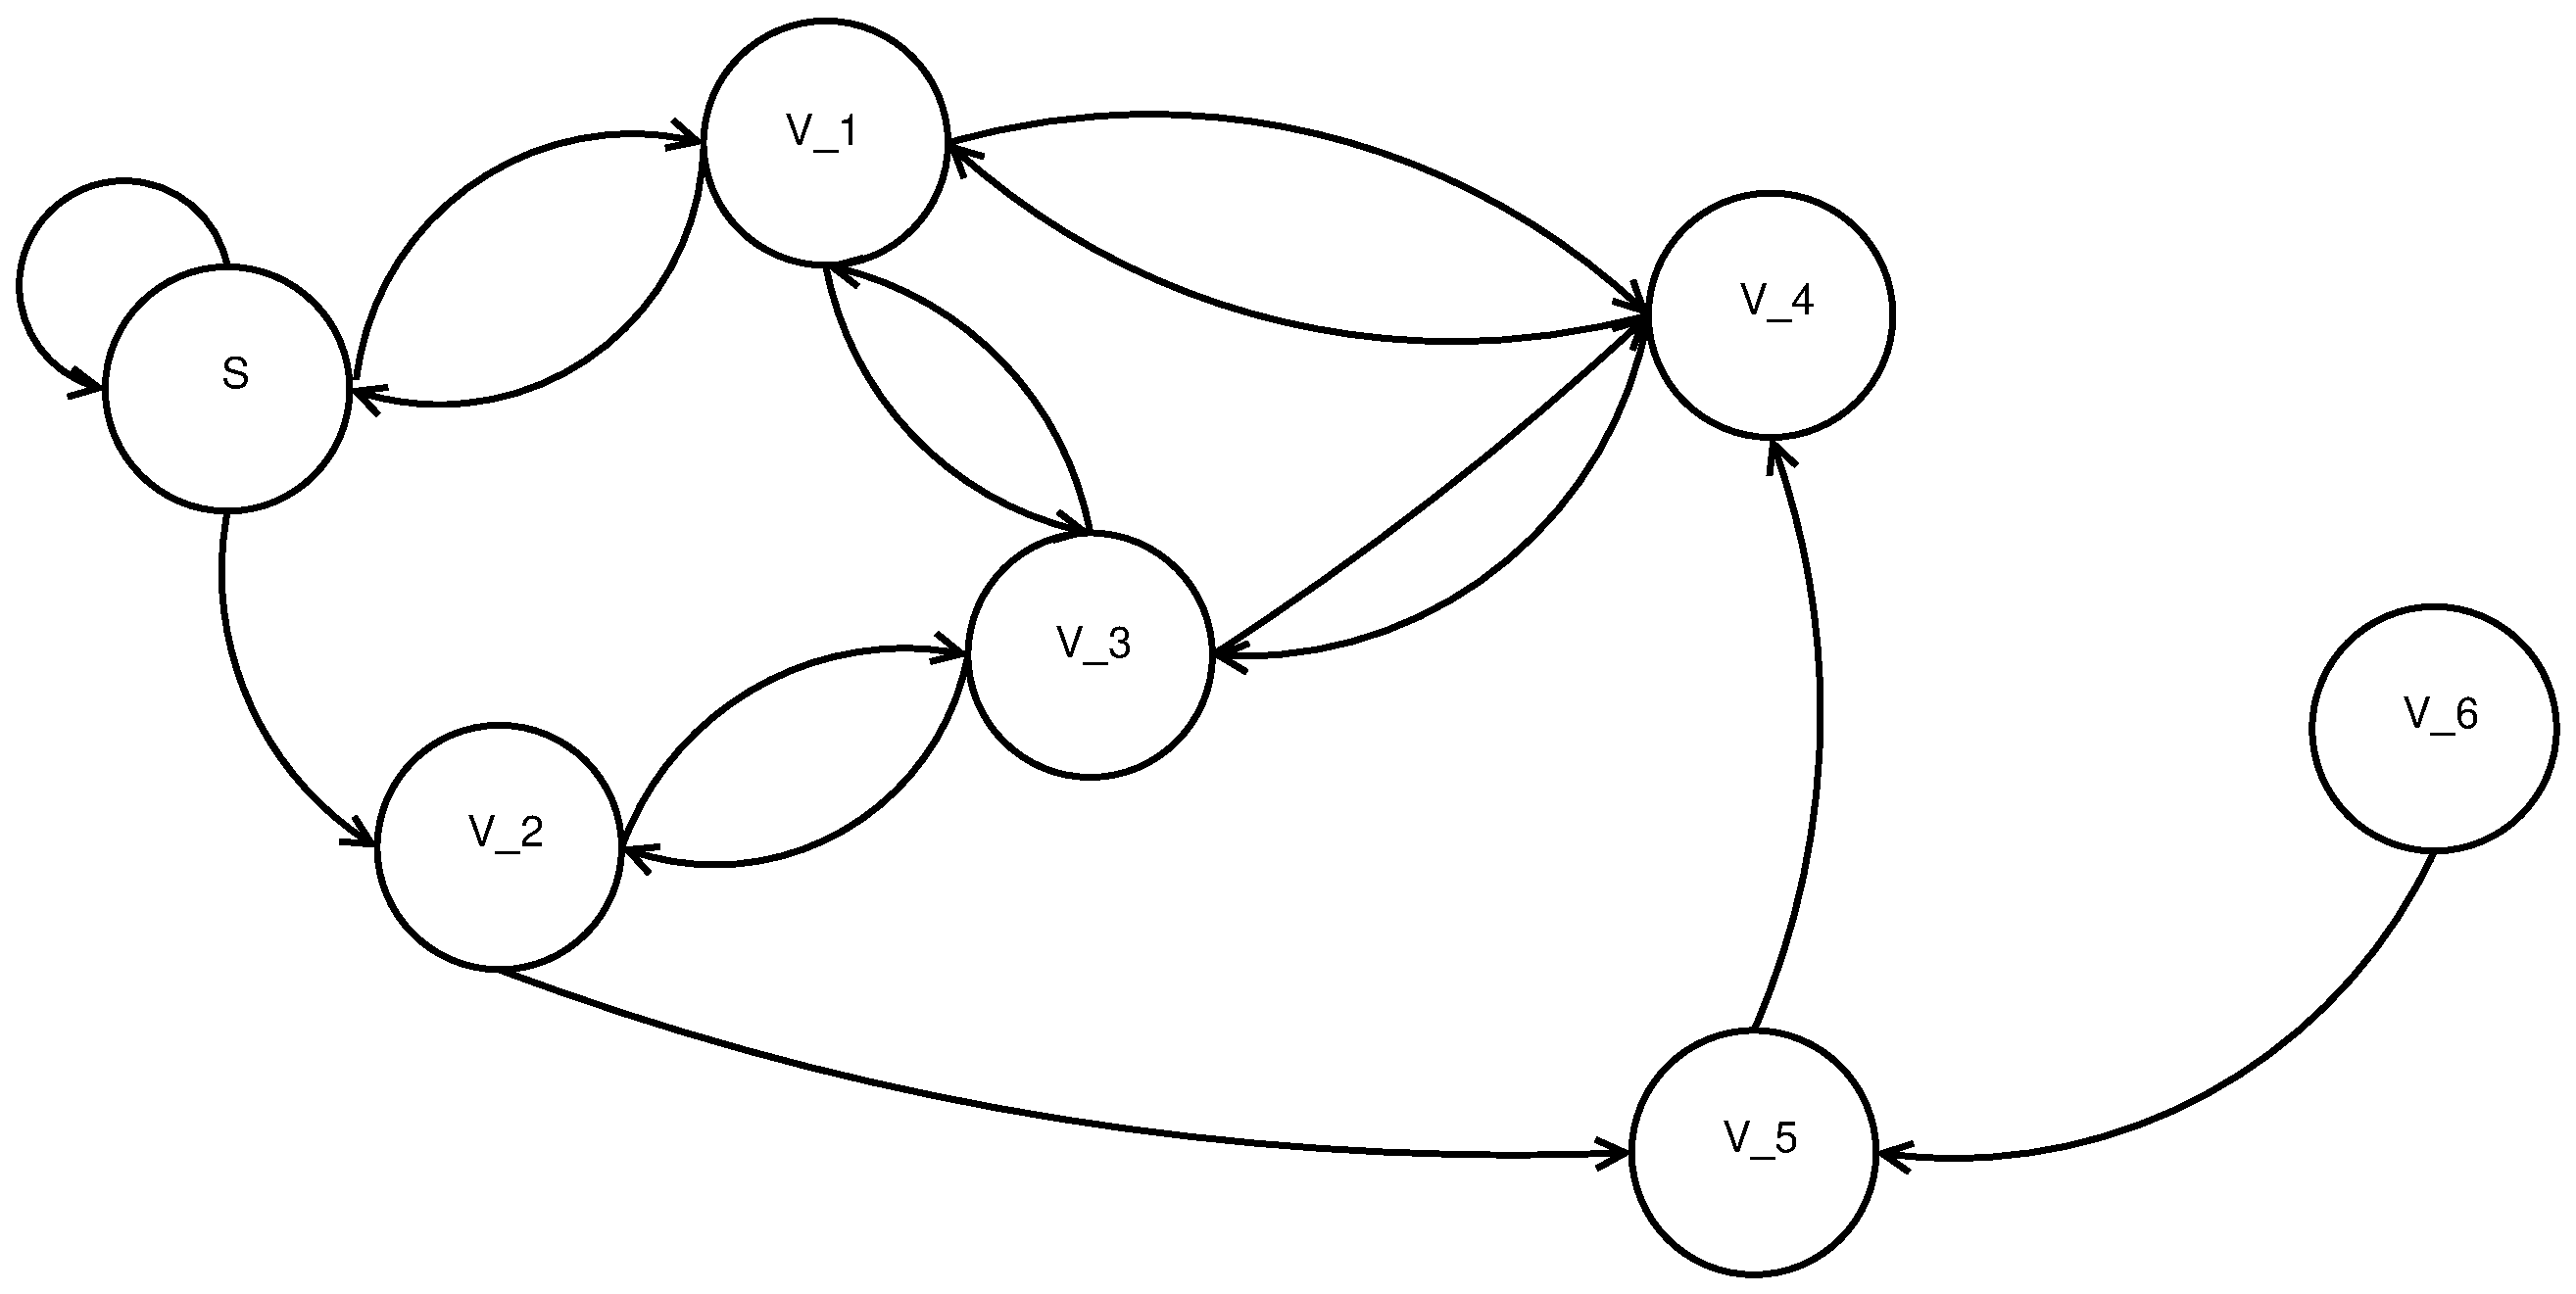
\includegraphics[width=0.5\linewidth]{15/Grafik/GerichteterGraph}
\caption{Gerichteter Graph}
\label{fig:GerichteterGraph}
\end{figure}

Planare Graphen können ohne Überkreuzung der Kanten in die Ebene eingebettet werden.

\subsubsection{Eulerische Polyederformel}
\begin{wrapfigure}{r}{0.25\linewidth}
	\centering
	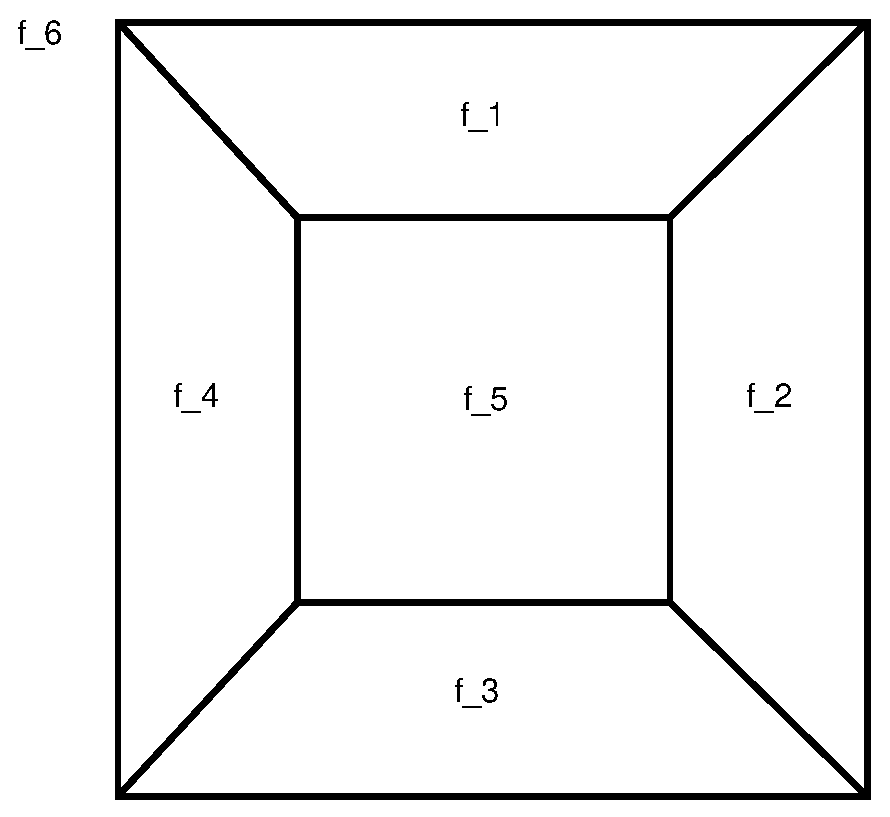
\includegraphics[width=\linewidth]{15/Grafik/Polyeder}
	\caption{Würfel}
	\label{fig:Polyeder}
	\vspace{-500pt}
\end{wrapfigure}

\[ |V| + |F| = |E| + 2 \]
\[ 8+6 = 12 + 2 \]
Es gilt: 
\[  2\cdot|E| \geq 3\cdot |F| \]
\begin{wrapfigure}{r}{0.25\linewidth}
	\vspace{-20pt}
	\centering
	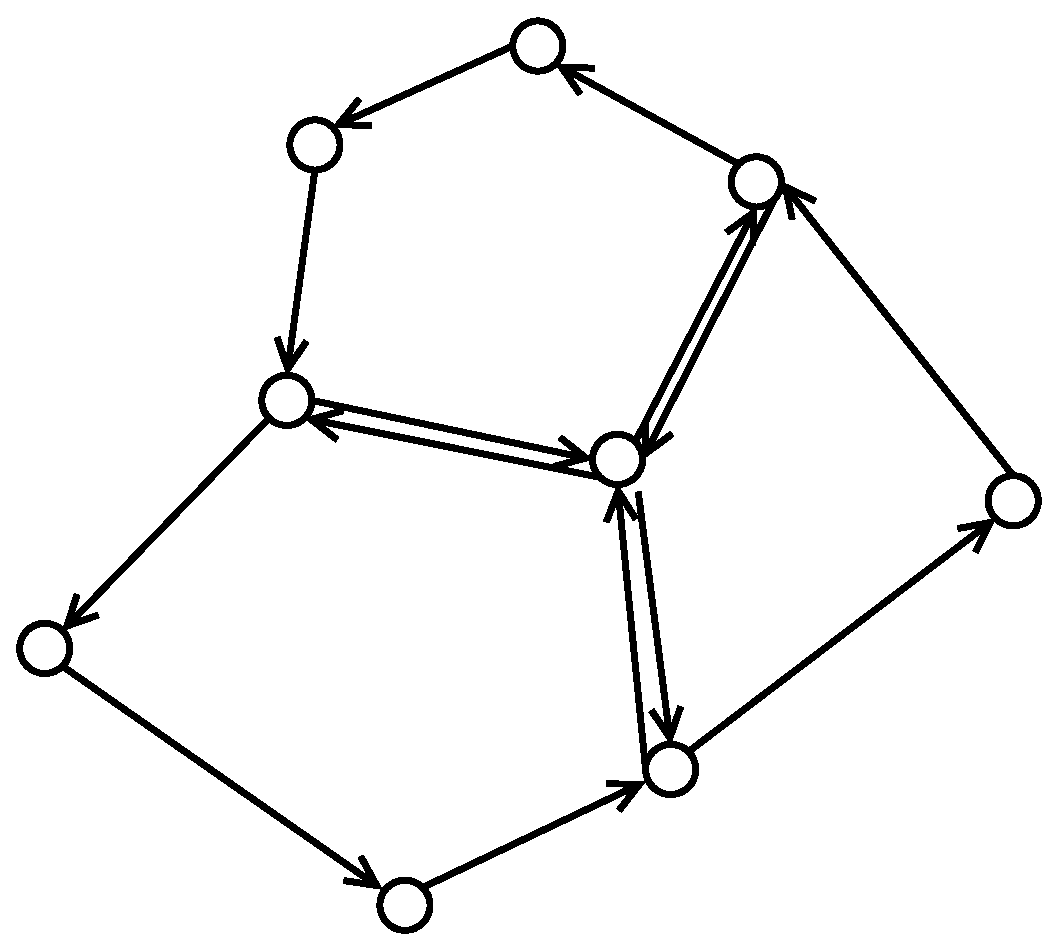
\includegraphics[width=\linewidth]{15/Grafik/Graph1}
	\caption{Placeholder}
	\label{fig:Graph1}
\end{wrapfigure}
\[ \text{\#gerichtete Kanten}= 2\cdot |E| = \sum_{i=1}^{|F|}\text{\#Kanten}(f_i)\footnote{Jedes $f_i$ hat mindestens 3 Kanten} \geq 3\cdot|F| \]
\[ |F| \leq \frac{2}{3}|E|,~~|V|+|F| = |E|+2\leq |V|+\frac{2}{3}|E| \Rightarrow \frac{1}{3}|E|+2 \leq |V|\]
\framebox{$\Rightarrow |E| \leq 3\cdot |V| -6$}
\begin{figure}[H]
\centering
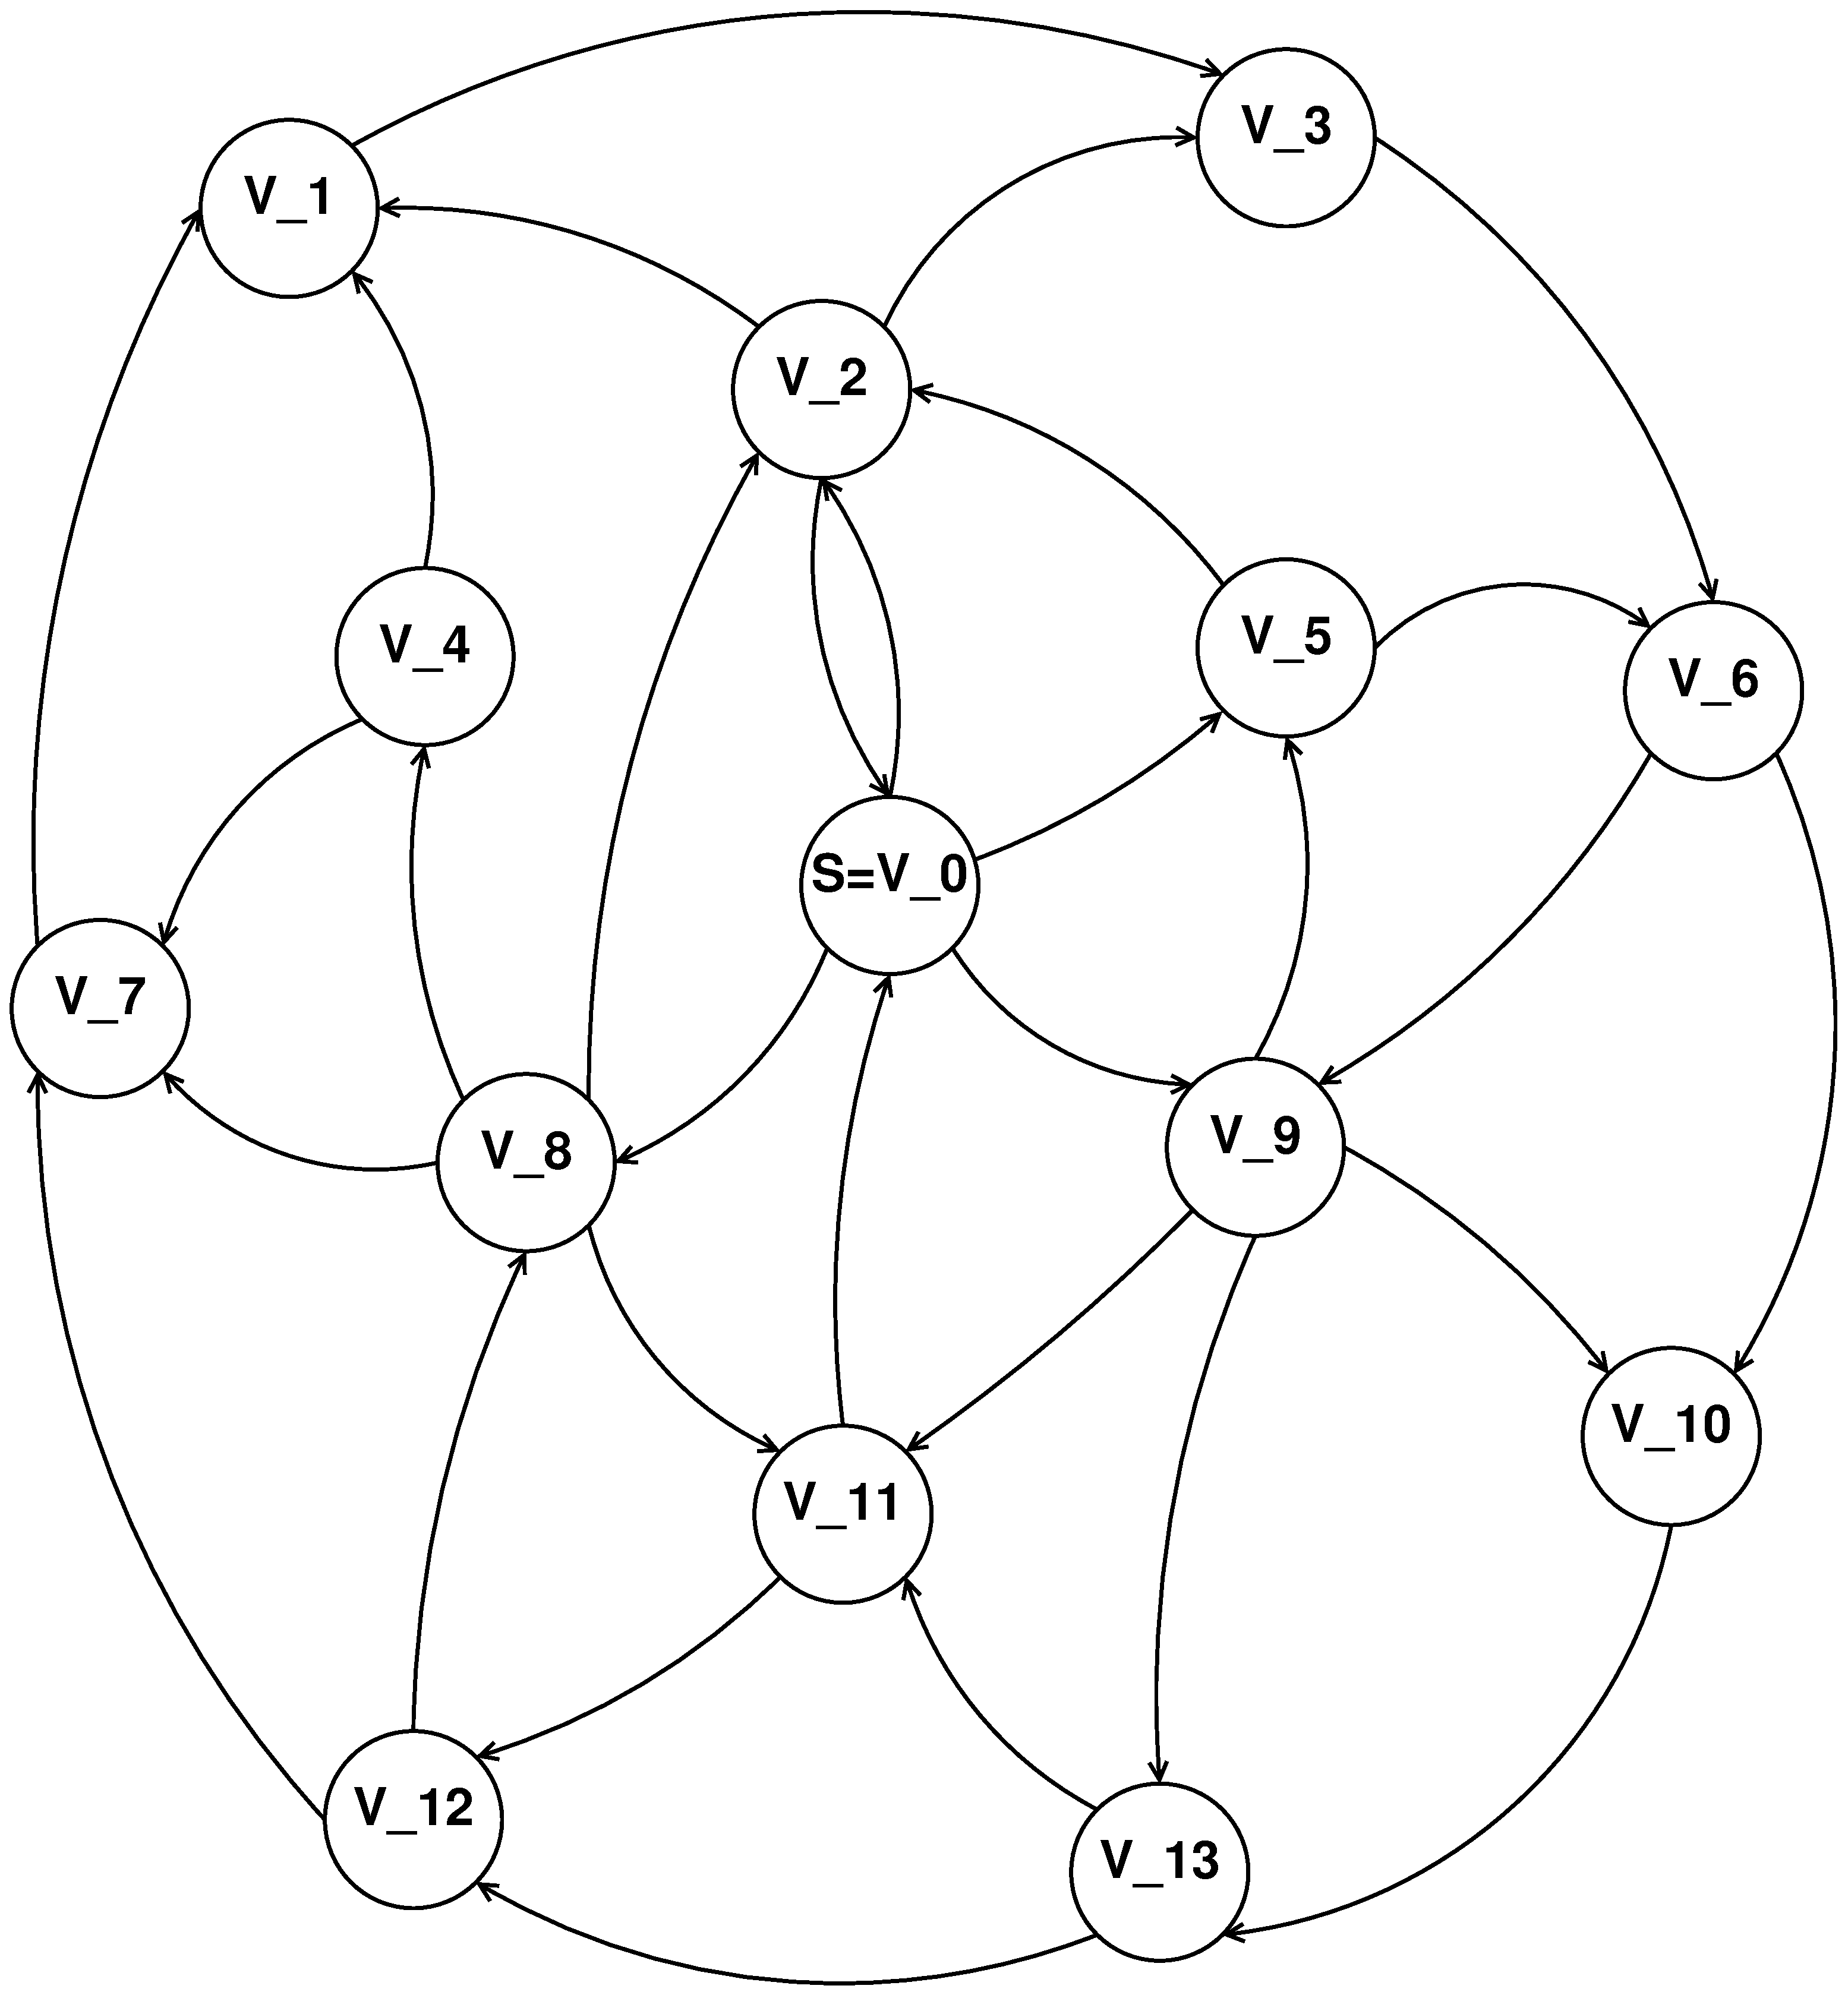
\includegraphics[width=0.5\linewidth]{15/Grafik/GerichteterGraph2}
\caption{Beispiel}
\label{fig:GerichteterGraph2}
\end{figure}

\subsubsection{Adjazenzmatrix}
\begin{tabular}{|c|cccccccccccccc|}
	\hline
	  &0&1&2&3&4&5&6&7&8&9&10&11&12&13 \\ \hline
	 0&1&0&1&0&0&1&0&0&1&1& 0& 0& 0& 0 \\
	 1&0&1&0&0&0&0&0&0&0&0& 0& 0& 0& 0 \\
	 2&1&1&1&1&0&0&0&0&0&0& 0& 0& 0& 0 \\
	 3&0&0&0&1&0&0&1&0&0&0& 0& 0& 0& 0 \\ \hline
	 4&0&1&0&0&1&0&0&1&0&0& 0& 0& 0& 0 \\ 
	 5&0&0&1&0&0&1&1&0&0&0& 0& 0& 0& 0 \\
	 6&0&0&0&0&0&0&1&0&0&1& 1& 0& 0& 0 \\
	 7&0&1&0&0&0&0&0&1&0&0& 0& 0& 0& 0 \\ \hline
	 8&0&0&1&0&1&0&0&1&1&0& 0& 0& 0& 0 \\
	 9&0&0&0&0&0&1&0&0&0&1& 1& 1& 0& 1 \\
	10&0&0&0&0&0&0&0&0&0&0& 1& 0& 0& 1 \\
	11&1&0&0&0&0&0&0&0&0&0& 0& 1& 1& 0 \\ \hline
	12&0&0&0&0&0&0&0&1&1&0& 0& 0& 1& 0 \\
	13&0&0&0&0&0&0&0&0&0&0& 0& 1& 1& 1 \\ \hline
	
\end{tabular}$= A$
\[ a\in B^{|V|\times |V|} \]
falls $G$ ungerichtet $\Rightarrow A = A^T$
\subsubsection{Adjazenzlisten Repräsentation}
\begin{figure}[H]
\centering
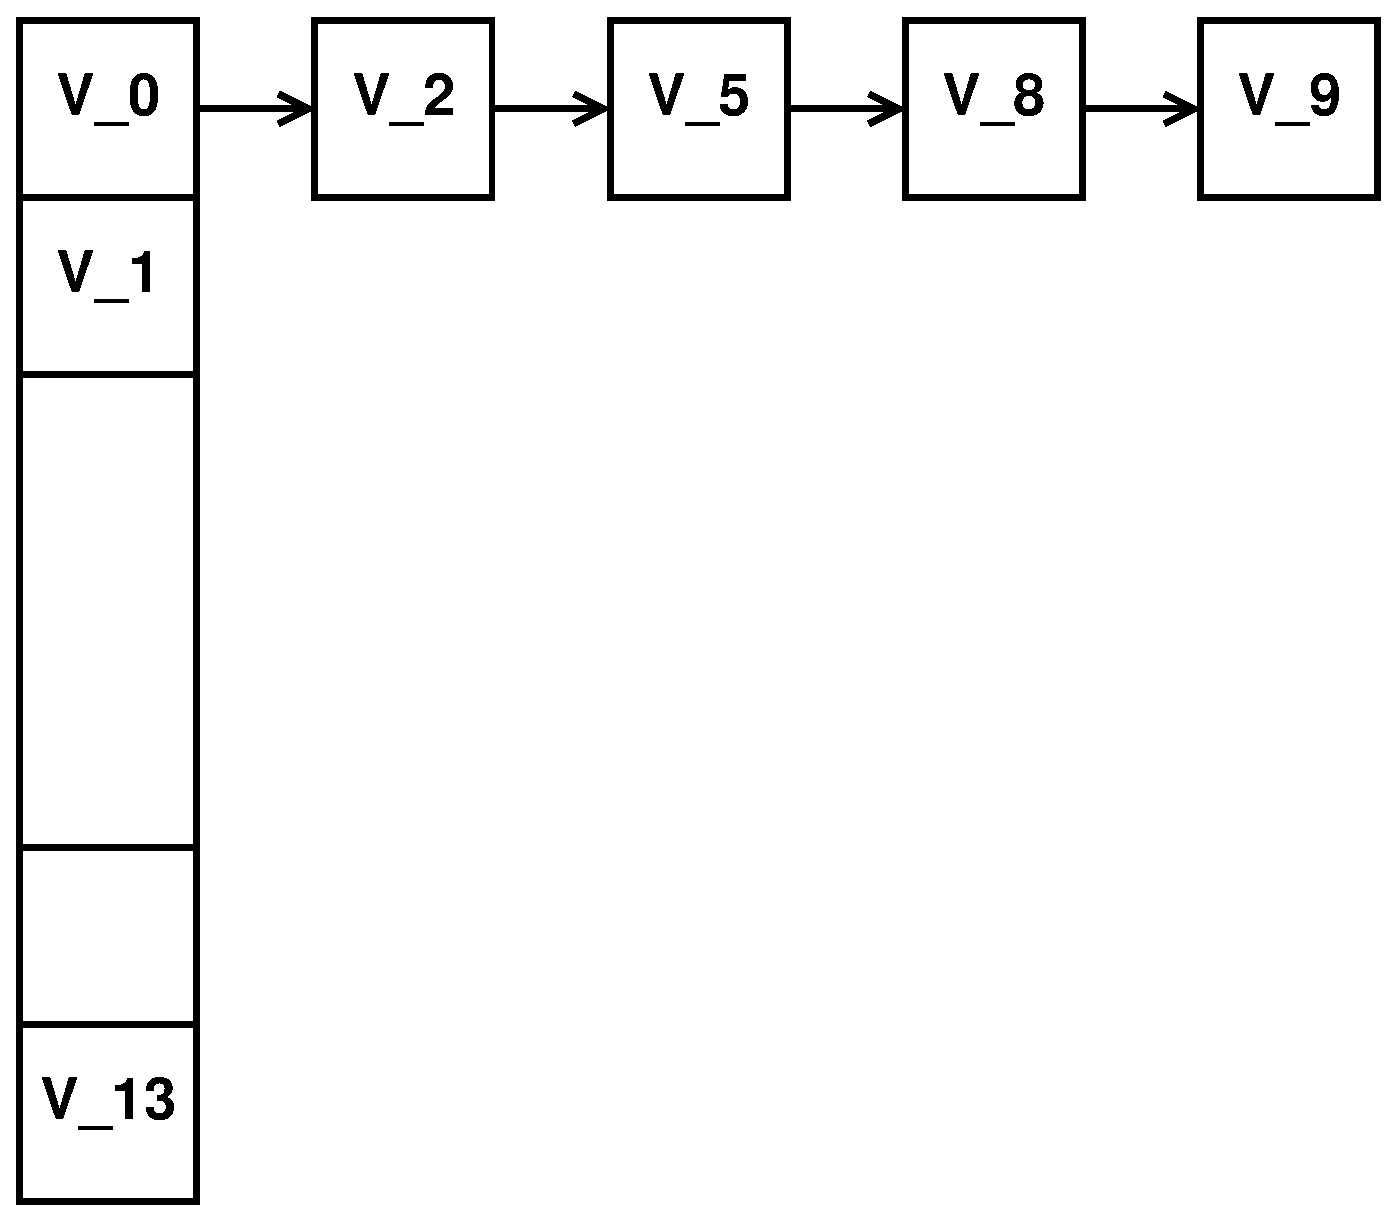
\includegraphics[width=0.4\linewidth]{15/Grafik/Liste}
\caption{Adjazenzliste}
\label{fig:Liste}
\end{figure}


\paragraph{Platzbedarf}
\[ \mathcal{O}(|V|+|E|)=\mathcal{O}\left( |V|+\sum_{i=0}^{|V|-1}\text{outdeg}(v_i) \right) \]
\begin{figure}[h]
\centering
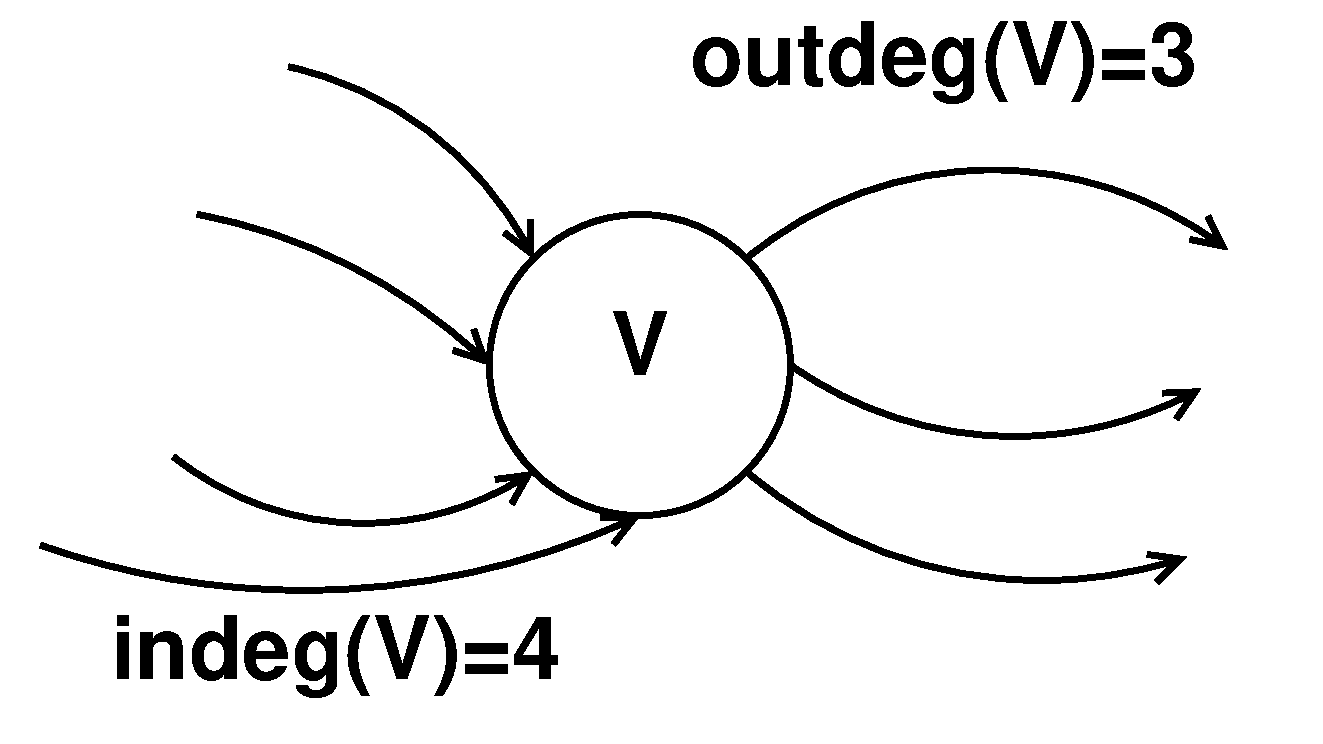
\includegraphics[width=0.3\linewidth]{15/Grafik/deg}
\caption{indeg und outdeg}
\label{fig:deg}
\end{figure}

\subsection{BFS (Breadth-First Search) Breitensuche}
\paragraph{Initialisierung}
\begin{lstlisting}
forall ( v in V\{S}) {
  col[v]=white;    // Farbe  weiß = unbekannt, grau = bekannt, schwarz = vollkommen bekannt
  d[v] = infinity; // Distanz
  pi[v] = NULL;    // pi ist Vorgänger
}
col[s] = grey;     // s ist Startknoten
d[s] = 0;
pi[s] = null;
\end{lstlisting}
\begin{tabular}{ccc}
	Queue & vs & Stack \\
	Schlange &$~$& Stapel \\
	empty() &$~$ & '' \\
	push() &$~$ & '' \\
	pop() &$~$ &  \\
	FIFO &$~$ & FILO \\
	First-In-First-Out &$~$& First-In-First-Out 
\end{tabular}
\begin{wrapfigure}{o}{0.4\textwidth}
	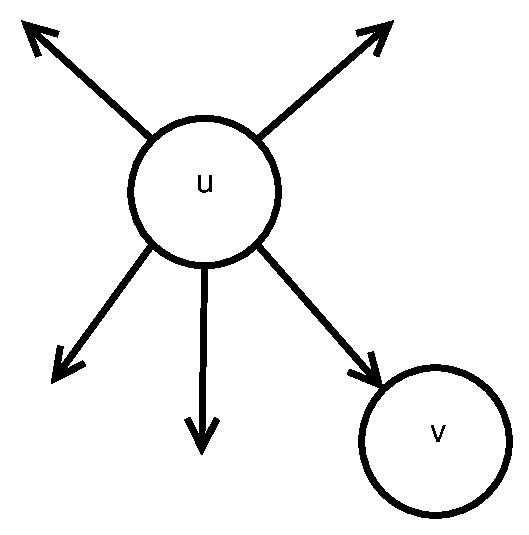
\includegraphics[width=\linewidth]{15/Grafik/CodeBild}
	\caption{Grafik zum Beispielcode}
	\label{fig:CodeBild}
\end{wrapfigure}
\begin{lstlisting}
Queue Q;
Q.push(s);
while(!Q.empty()) {
  u = Q.pop();
  forall( (u,v) in E) {
    if (col[v] == white) {
      col[v] == grey;
      d[v] = d[u]+1;
      pi[v] = u;
      Q.push(v);
    }
  }
  col[u] = black;
}
\end{lstlisting}

\paragraph{Laufzeit}
\[ \mathcal{O}(|V|+|E|) \]
\paragraph{Begründung:}
Jeder von $s$ aus erreichbare Knoten wird nur einmal in die Queue aufgenommen und auch ihr entfernt. Für jeden Knoten muss nur einmal seine Adjazenzliste durchlaufen werden.
\[  \Rightarrow \mathcal{O}\left(|V|+\sum_{v \in V}\text{outdeg}(v) \right) \]
\chapter{Vorlesung 16}

\begin{figure}[H]
\centering
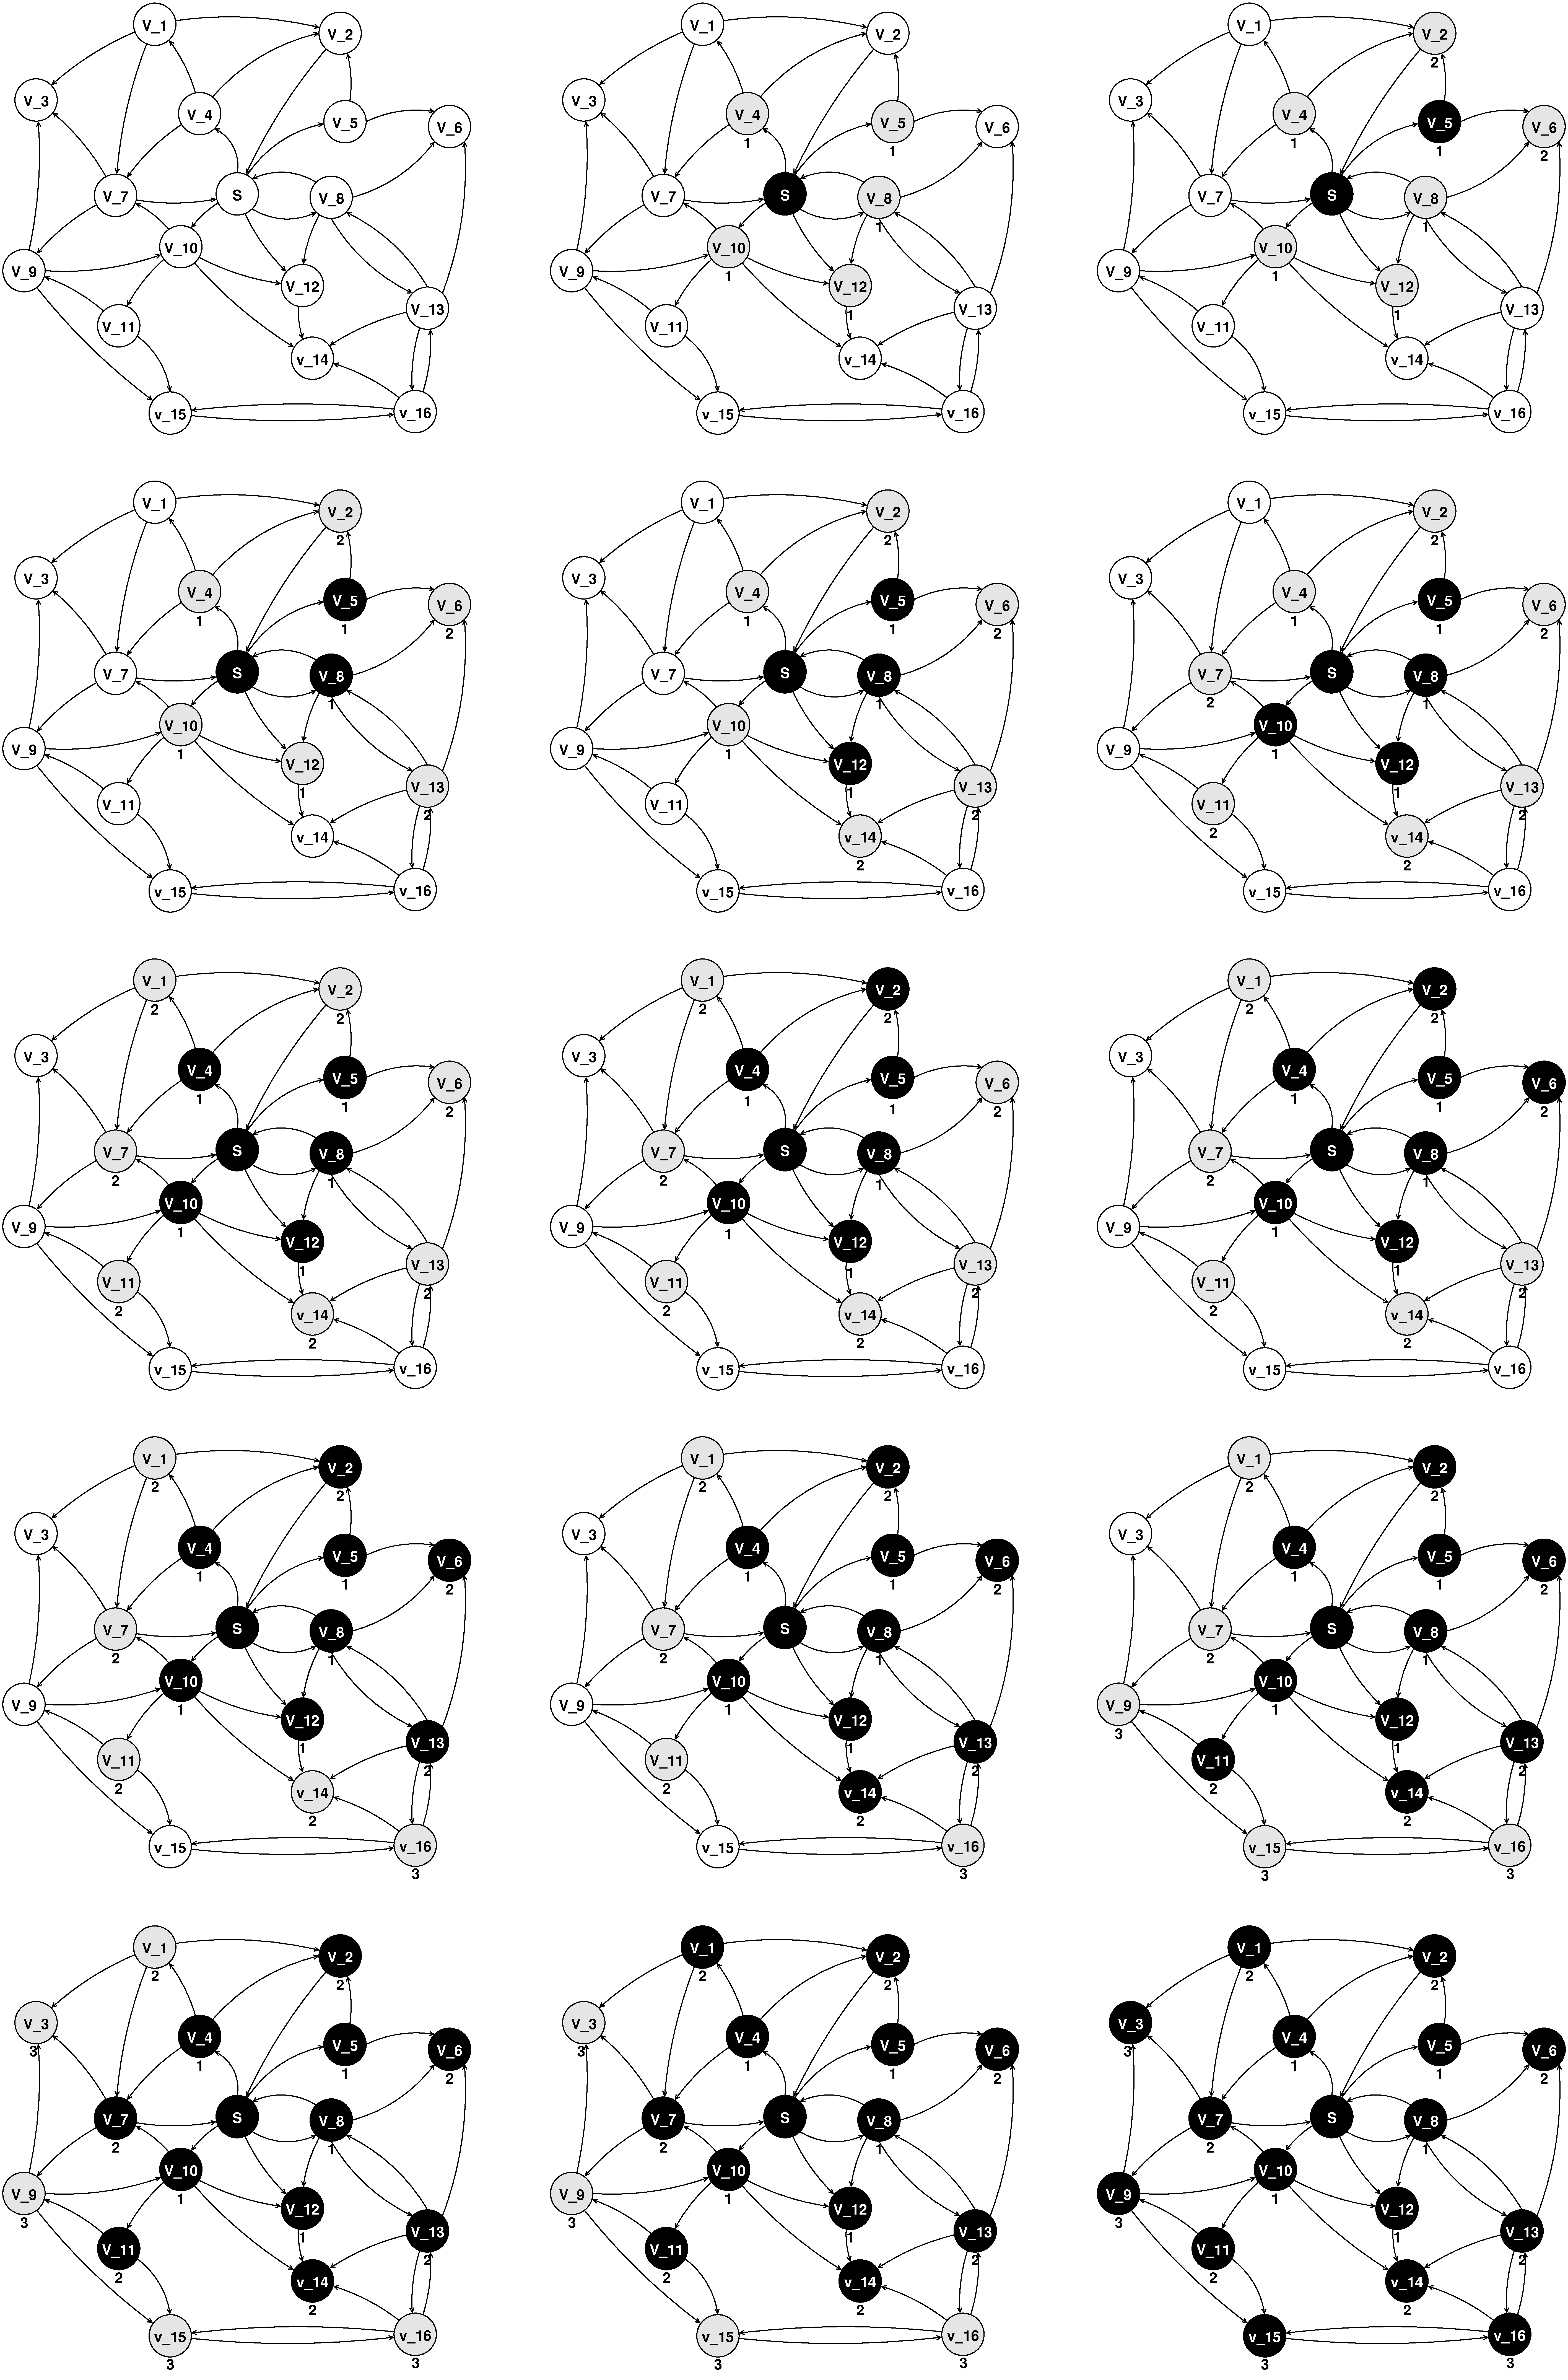
\includegraphics[width=0.9\linewidth]{16/Grafik/Diagramm}
\caption{Beispiel}
\label{fig:Diagramm}
\end{figure}


\subsubsection{Definition: Länge kürzesten Weges}
$\delta(s,v)=$ Länge eines kürzesten Weges vom Startknoten $s$ zum Knoten $v$.\\
Setze $\delta(s,v)=\infty$, falls v nicht erreichbar von s aus.
\subsubsection{Satz: Richtigkeit des Algorithmus}
Nach Ablauf von BFS\footnote{Breitensuche} gilt 
\[ \forall v\in V: ~ d[v]=\delta(s,v) \]
\subsubsection{Lemma 1: Dreiecksungleichung für kürzeste Wege}
\begin{figure}[h]
\centering
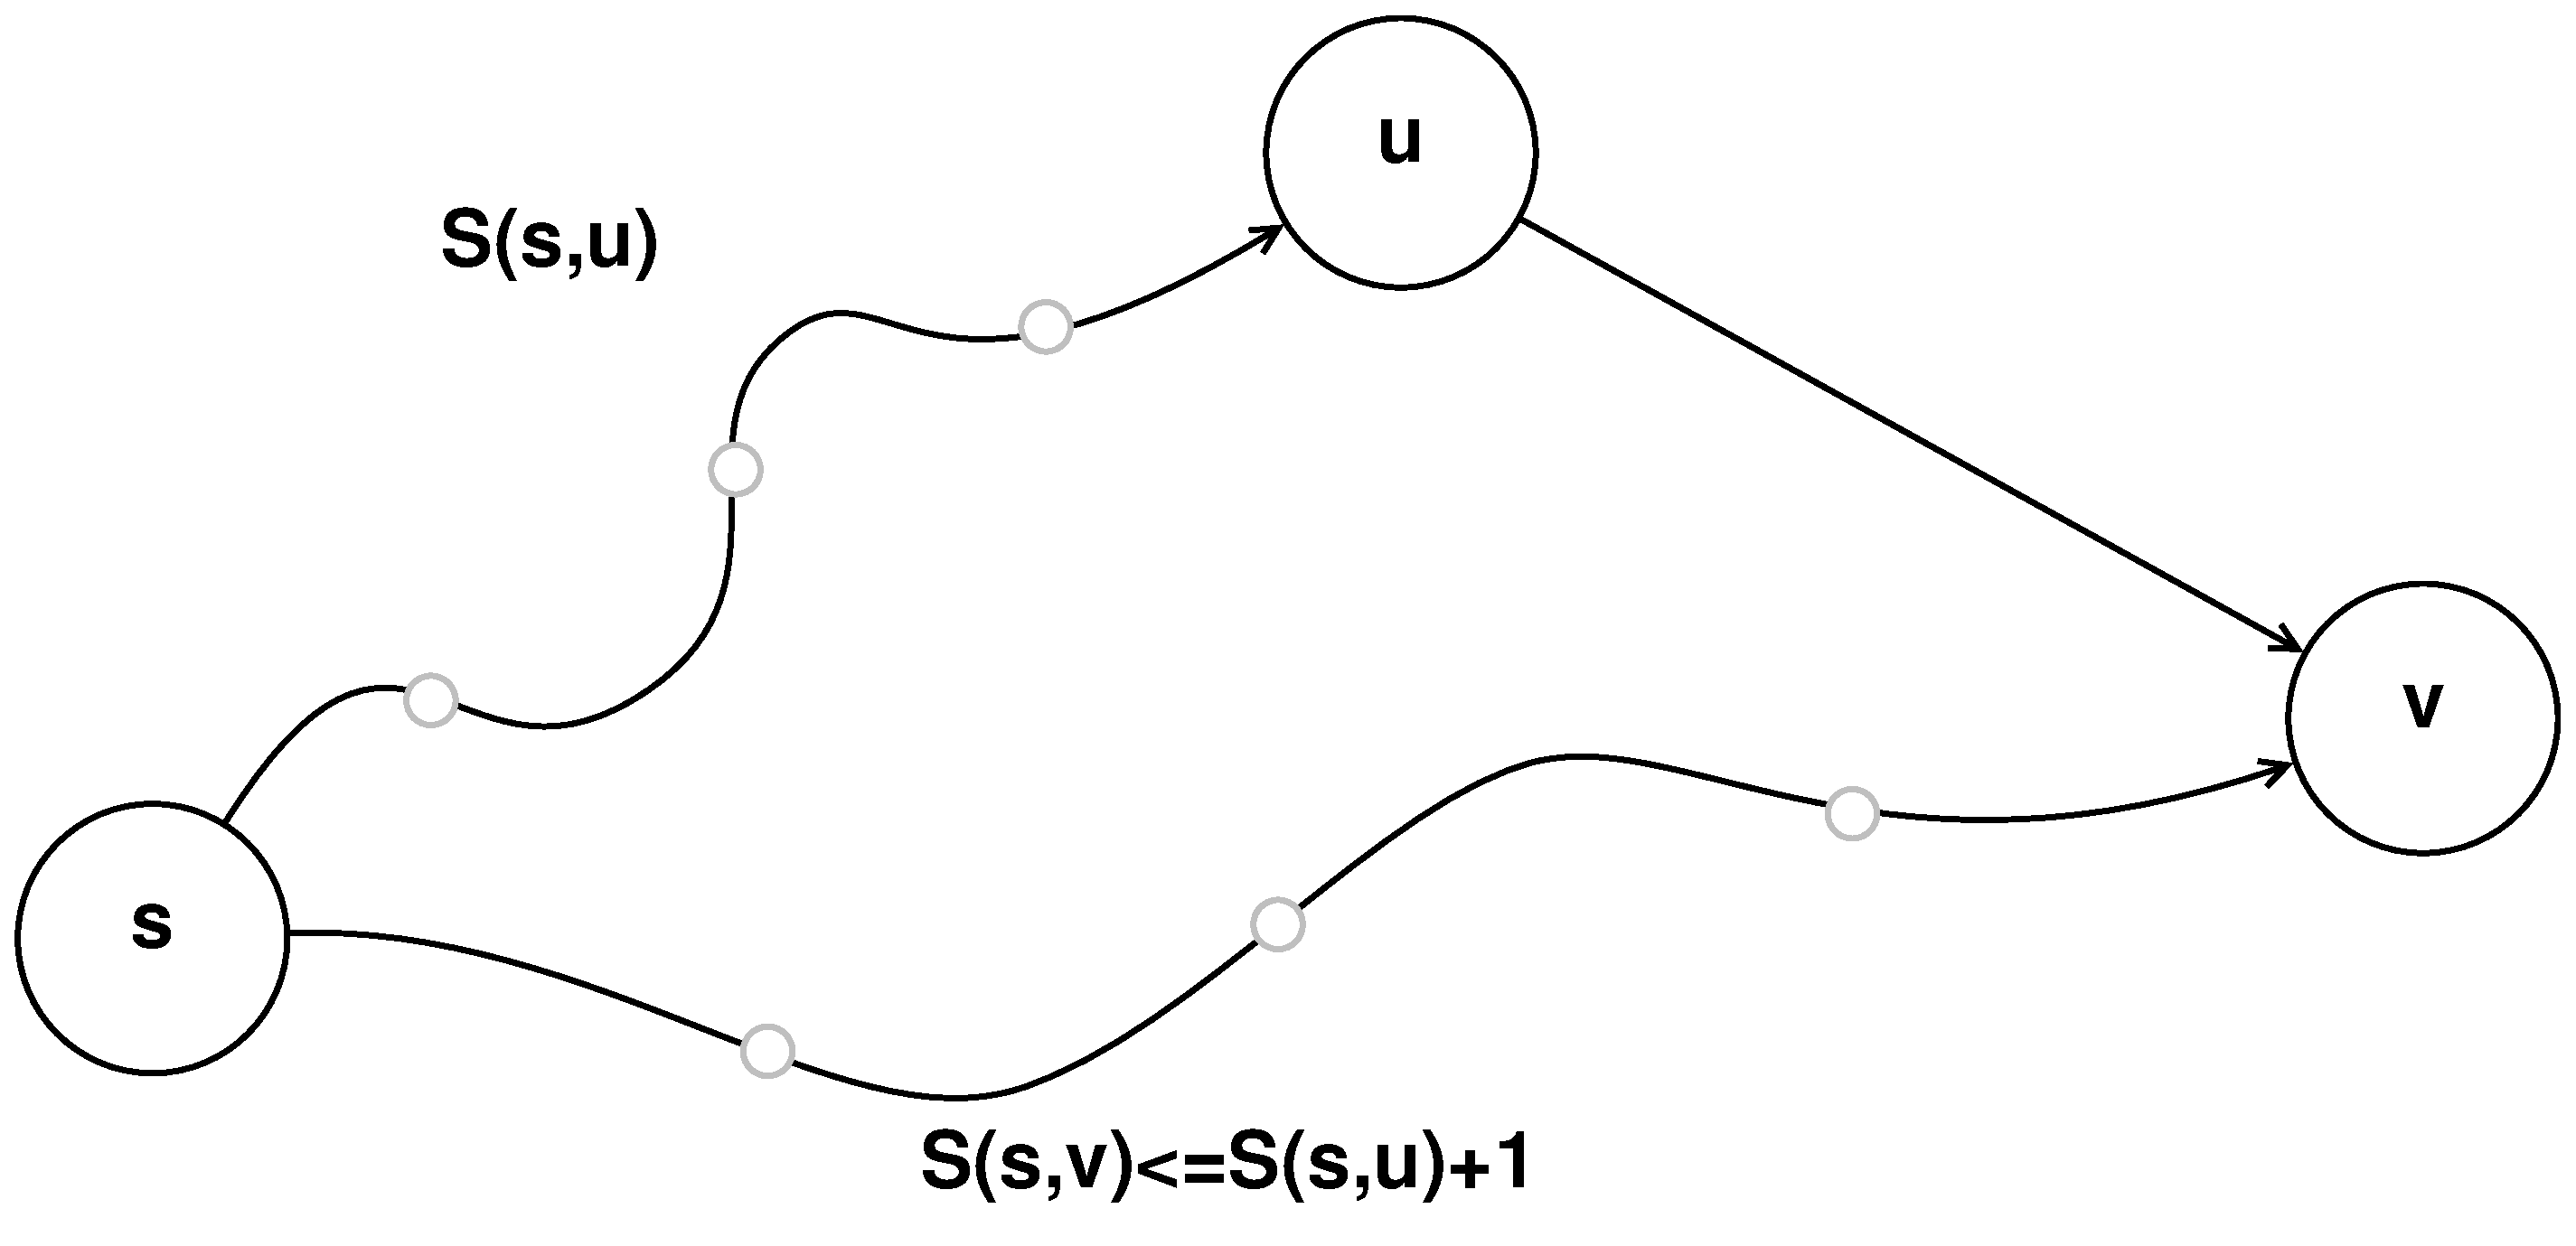
\includegraphics[width=0.7\linewidth]{16/Grafik/Dreiecksungleichung}
\caption{}
\label{fig:Dreiecksungleichung}
\end{figure}

\subsubsection{Lemma 2}
Zu jedem Zeitpunkt im Verlauf von BFS gilt:
\[ \forall v\in V:~ d[v] \geq \delta(s,v)\]
\subsubsection{Beweis (induktiv über Zahl der Operationen, die d-Wert verändern)}
\paragraph{Induktions-Anfang} \[ d[s] = 0 \surd\]
\paragraph{Induktions-Schritt} Knoten $v$ wird von $u$ aus neu entdeckt
\[ d[u]\geq \delta(s,u) \]
\[ d[v] = d[u]+1 \geq \delta(s,u)+1 \overset{D.U.}{\geq} \delta(s,v) \]
\subsubsection{Lemma 3}
Sei $Q=(v_1,v_2,\ldots,v_k)$ eine Queue, dann gilt stets:
\[ d[v_1]\leq d[v_2]\leq\ldots\leq d[v_k]\leq d[v_1]+1 \]
\subsubsection{Beweis (induktiv über die Zahl der push- und pop-Operationen)}
\paragraph{Induktions-Anfang}
\[ d[s] = 0 \surd\]
\paragraph{Induktions-Schritt}
\subparagraph{pop}
\[  \text{\sout{$d[v_1]$}}\leq d[v_2]\leq\ldots\leq d[v_k]\leq d[v_1]+1 \overset{!}{\leq} d[v_2]+1 \]
\subparagraph{push}
\[ d[u] = d[v_1]\leq d[v_2]\leq\ldots\leq d[v_k]\leq d[u]+1 \]
Beachte Kante $(u,v)$ $v$ ist weiß
\[ v=v_{k+1} \text{ wird gepushed} \]
\[ d[v_{k+1}] = d[v_1]+1 \]
Zustand von Q nach push
\[ d[v_2 \leq d[v_3] \leq\ldots\leq d[v_k]\leq d[v_1]+1 = d[v_{k+1}]~~\surd \]
\subsubsection{Satz: Richtigkeit des Algorithmus}
Nach Ablauf von BFS\footnote{Breitensuche} gilt 
\[ \forall v\in V: ~ d[v]=\delta(s,v) \]
\subsubsection{Beweis durch Widerspruch}
Sei $v\in V$, so dass $d[v] \neq \delta(s,v)$ am Ende des Algorithmus $\overset{Lemma2}{\Longrightarrow} d[v] > \delta(s,V)$\\
Sei $v$ so gewählt, dass es der erste knoten ist mit der Eigenschaft, dass sein d-Wert flasch gesetzt wird. d.h. Alle d-Werte bis zu diesem Zeitpunkt sind korrekt.\\
Sei $s\mapsto u'\rightarrow v$ ein kürzester Weg $s$ ui $v$\\
Betrachte die Situation bei Bearbeitung von $u'$:
\paragraph{1. Fall} $v$ ist in diesem Moment schwarz.
\[ d[v] > \delta(s,v)=\delta(s;u')+1\geq\footnote{$v$ vor $u'$ aus $Q$ entfernt und Lemma 3.} d[v]\lightning \]
\paragraph{2. Fall}
$v$ ist in diesem Moment weiß.
\[ d[v]>\delta(s,u')+1=d[u']+1=\footnote{wegen Wahl von $v$; d-Wert von $u'$ muss also korrekt sein}d[v] \lightning \]
\clearpage
\paragraph{3. Fall}
\begin{wrapfigure}{r}{0.4\linewidth}
	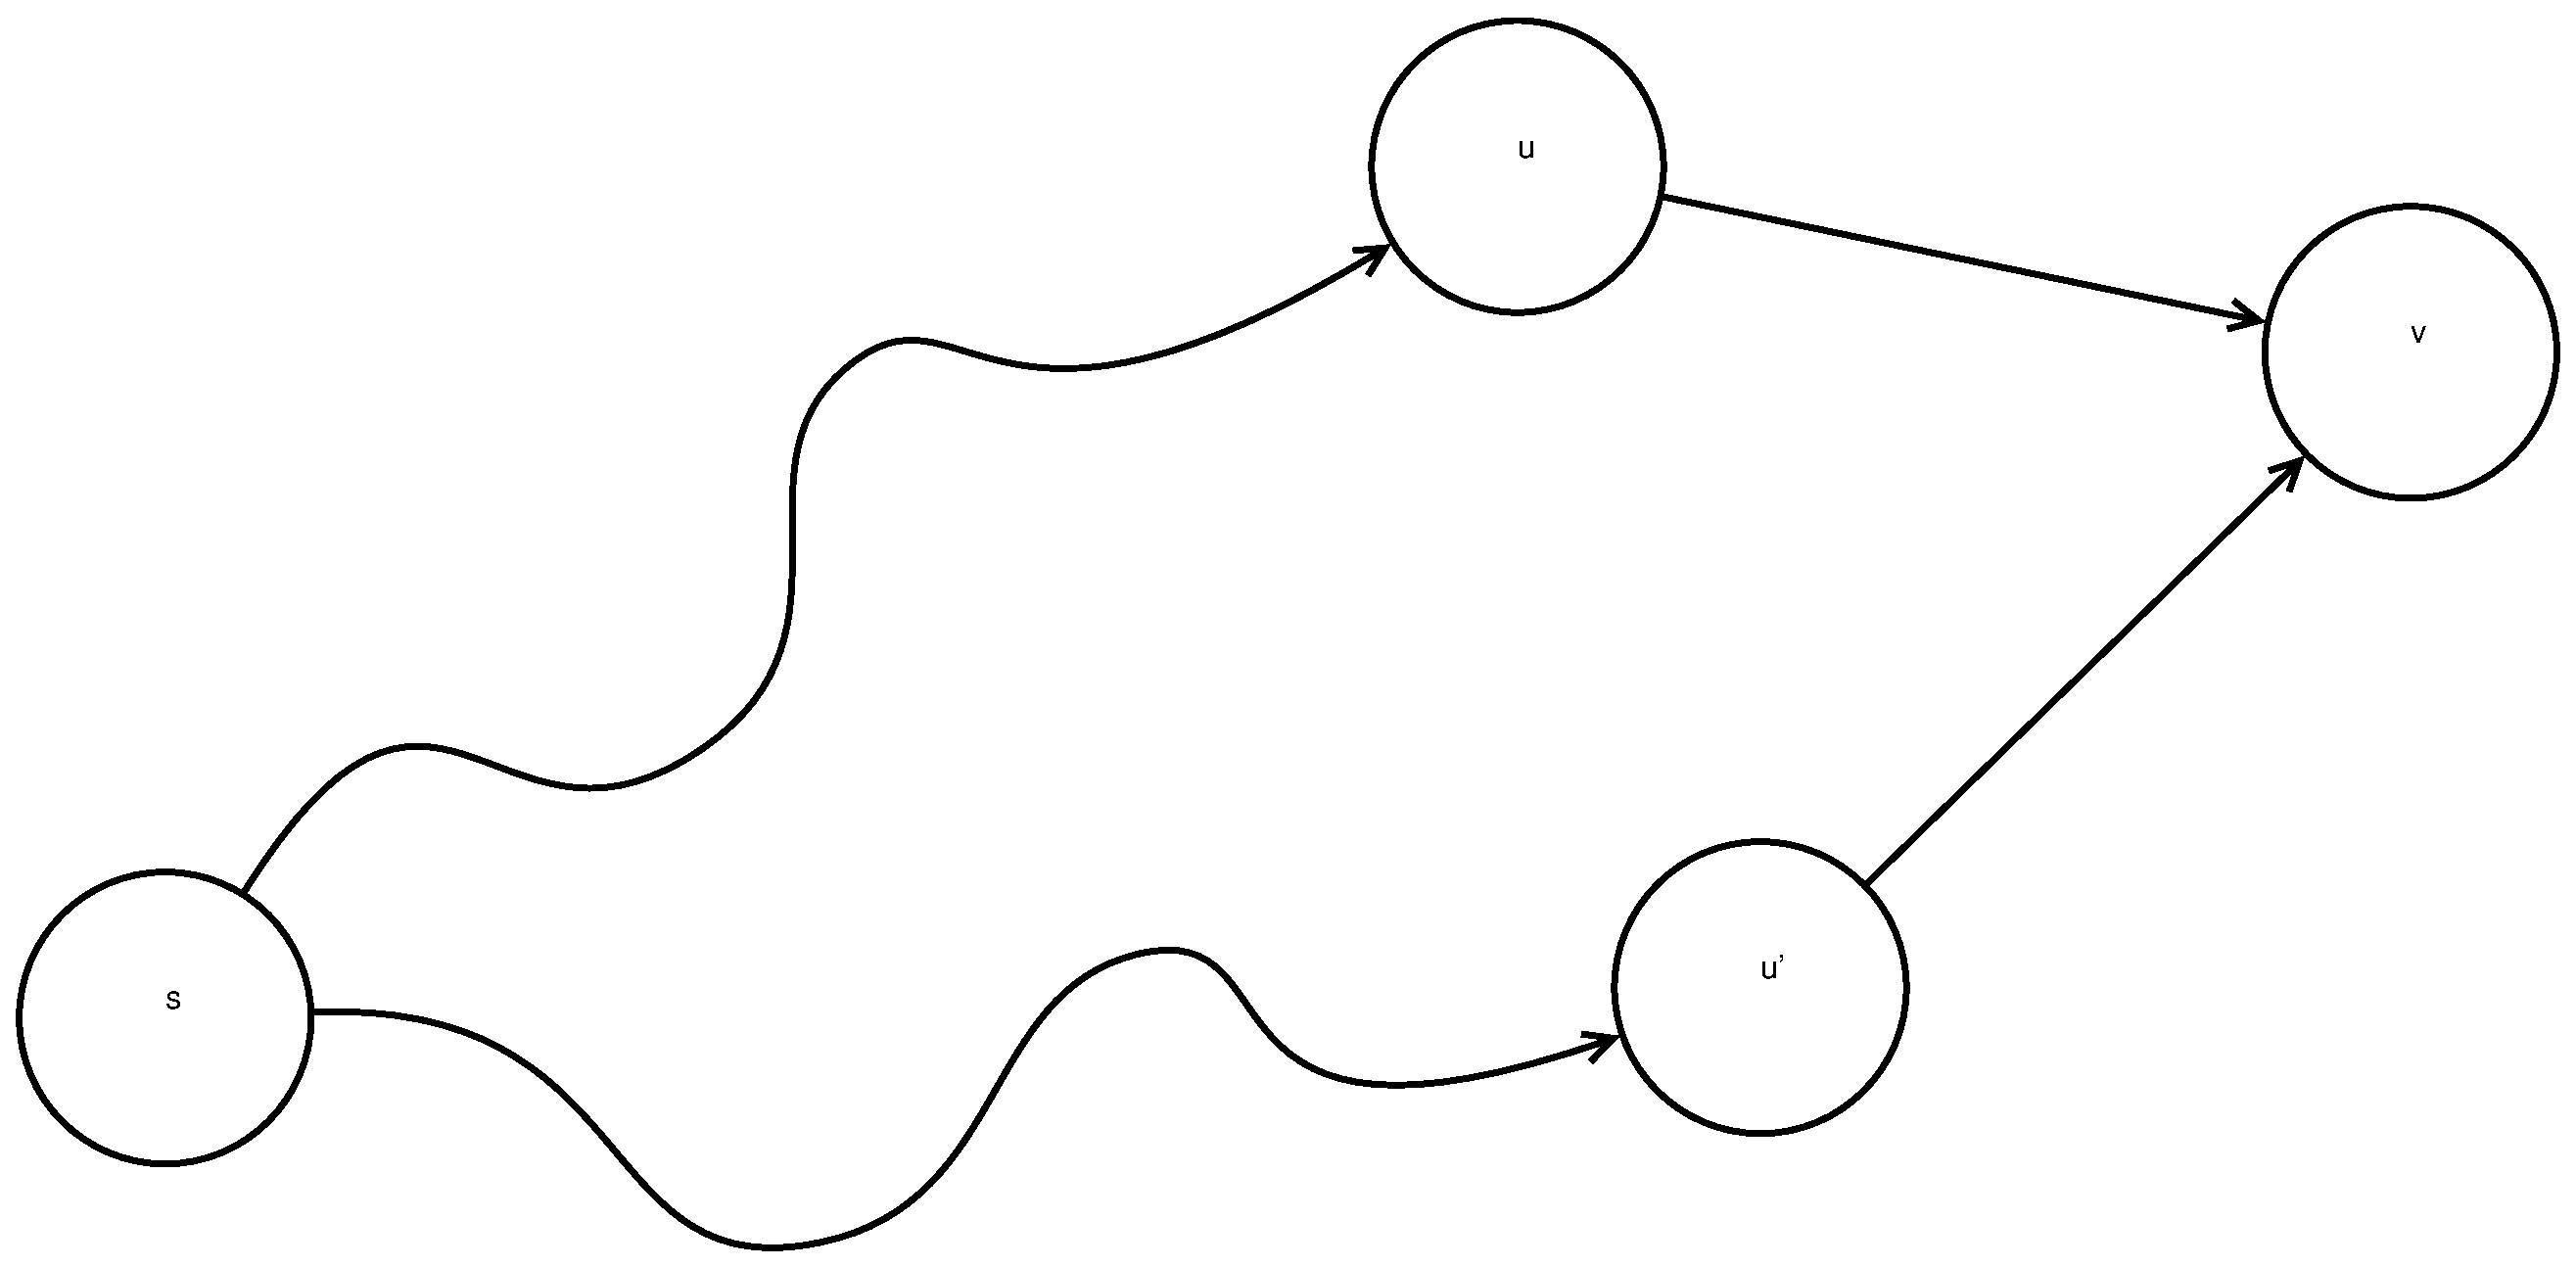
\includegraphics[width=\linewidth]{16/Grafik/Beweis}
	\caption{}
	\label{fig:Beweis}
\end{wrapfigure}
$v$ ist grau.
\[ d[v]>\delta(s,u')+1=d[u']+1\geq d[u]+1=d[v] \]
$d[u]\leq d[u']$, weil $u$ vor $u'$ aus $Q$ entfernt $\lightning$
\begin{flushright}
	q.e.d.
\end{flushright}
\section{Kürzeste Wege Algorithmen}
\subsection{Dijkstra-Algorithmus}
\[ G=(V,E)~~w:E\rightarrow \mathbb{R}^+_0 \]
\begin{figure}[h]
\centering
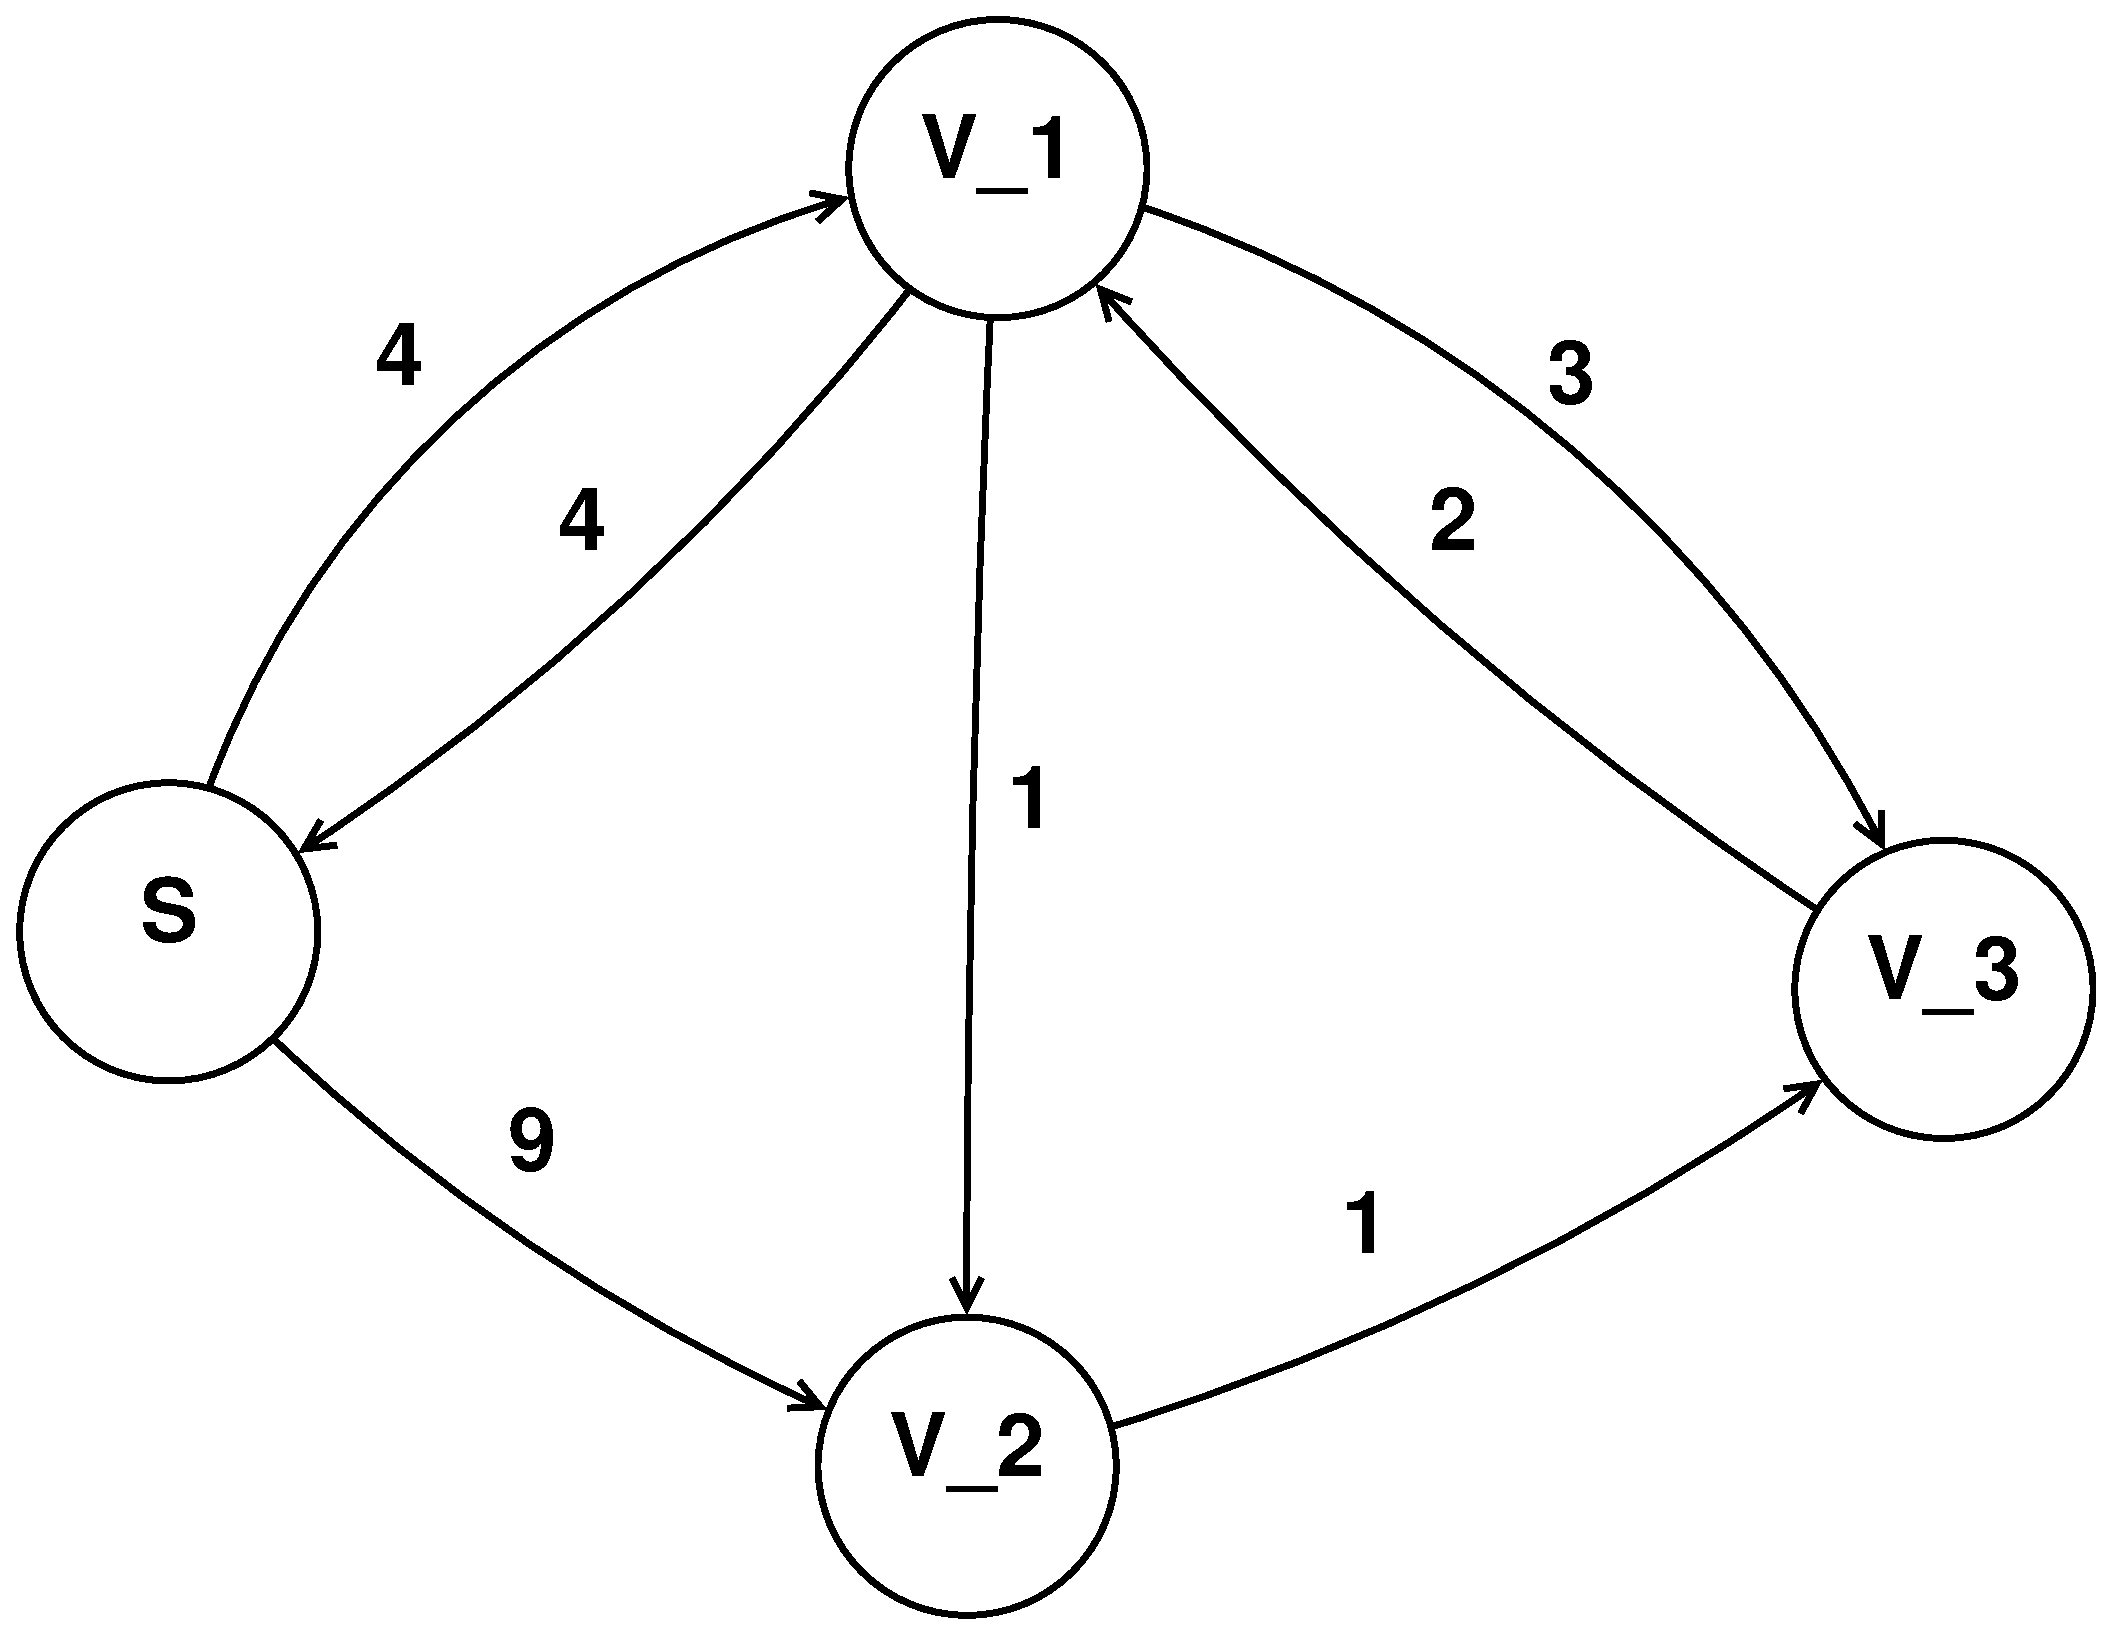
\includegraphics[width=0.3\linewidth]{16/Grafik/Dijkstra}
\caption{}
\label{fig:Dijkstra}
\end{figure}

Sei $p=(s=v_0,v_1,v_2,\ldots,v_k)$
\begin{figure}[h]
	\centering
	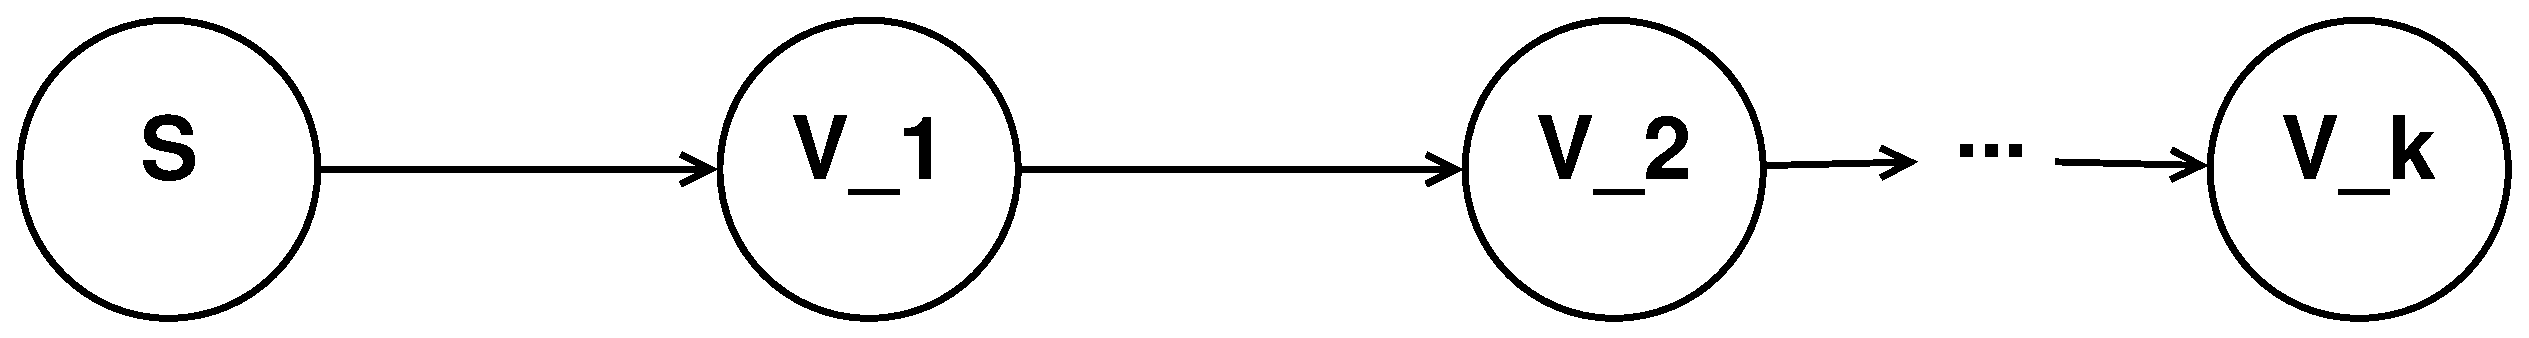
\includegraphics[width=0.3\linewidth]{16/Grafik/Dijkstra2}
	\caption{}
	\label{fig:Dijkstra2}
	\end{figure}
\[ w(p) = \sum_{i=0}^{k-1}w(v_i,v_{i+1})=\delta(s,v_k) \]
\begin{figure}[h]
	\centering
	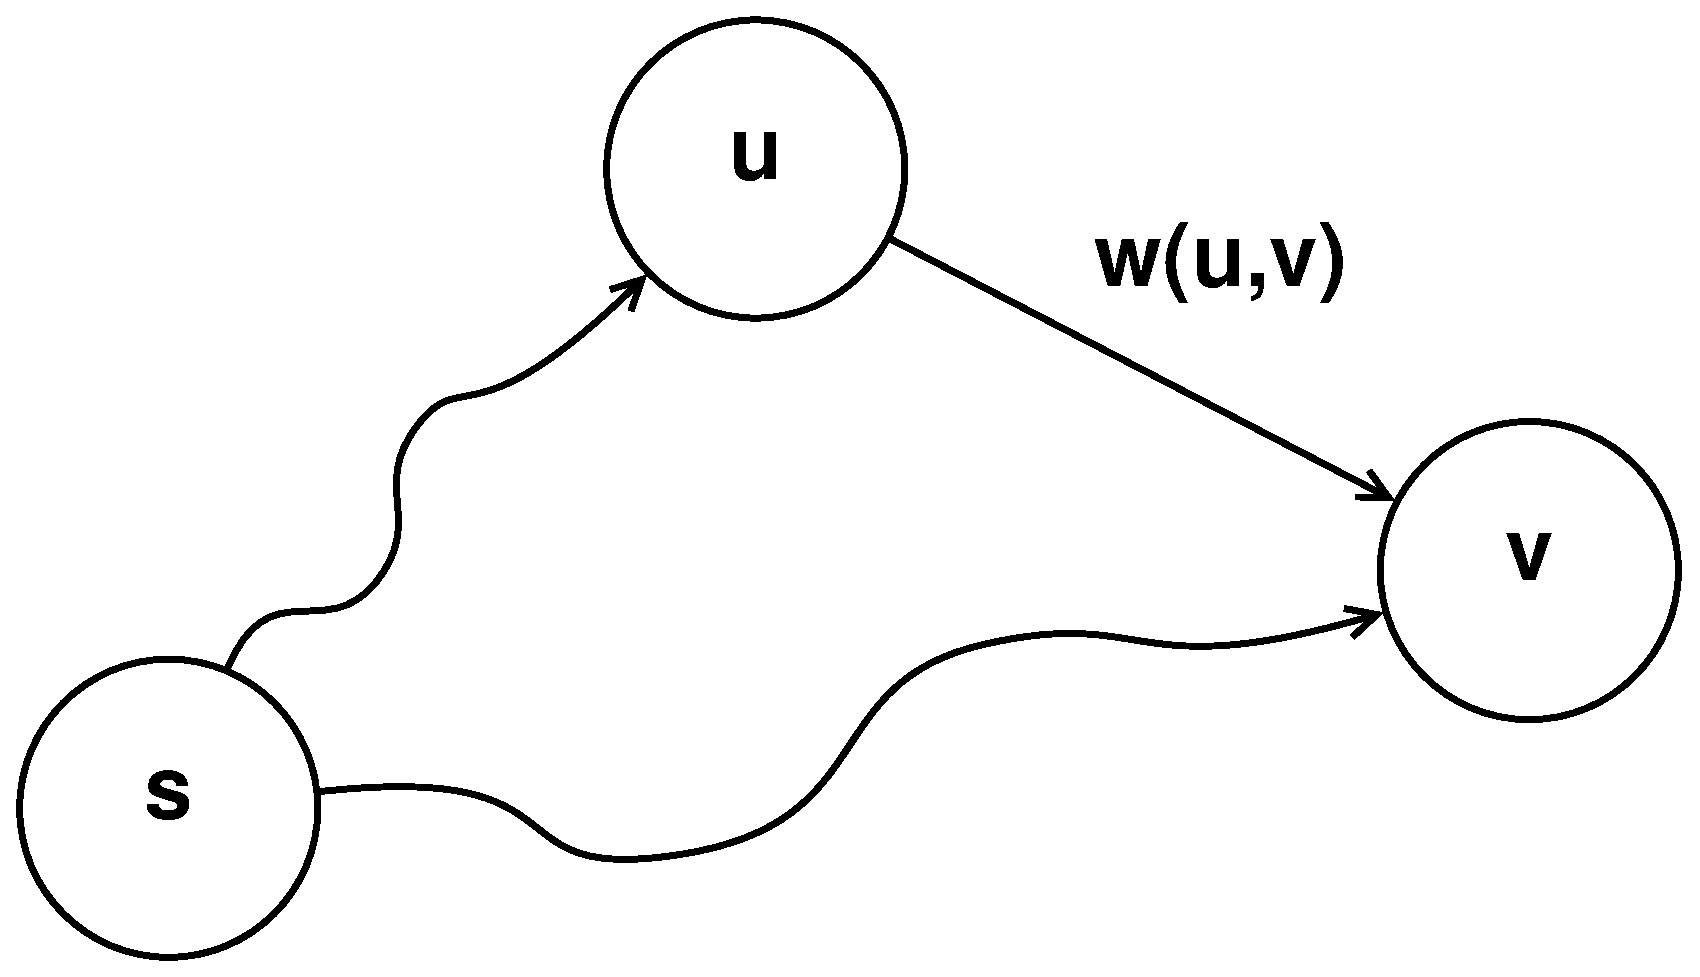
\includegraphics[width=0.3\linewidth]{16/Grafik/dijkstra3}
	\caption{}
	\label{fig:Dijkstra3}
	\end{figure}
\[ \delta(s,v)\leq \delta(s,U)+w(u,v) \]
\begin{lstlisting}
relax(u,v,w) {
  if(d[v] > d[u]+w(u,v) ) {
    d[v] = d[u] + w(u,v);
    /pi[v] = u;
  }
}
\end{lstlisting}
Betrachte Algorithmen zur kürzesten Wege Berechnung, die Distanzwerte nur mit Hilfe dieser relax-Funktion verändern, dann gilt:
\[ d[v] \geq \delta(s,v)~~\forall v\in V \]
\paragraph{Beweis}
\[ d[v] = d[u]+w(u,v) \overset{I.A.}{\geq} \delta(s,u)+w(u,v) \geq \delta(s,v) \]
Induktion über Zahl der reflex-Aufrufe

\end{document}